\RequirePackage{graphicx} 
%In draft mode, display low-res figures
%add `draft` parameter, for placeholders of figs
%https://tex.stackexchange.com/a/74901/199031

%%%%%%%%%%%%%%%%%%%%%%%%%%%%%%%%%%%%%%%%%%%%%%%%%%%%%%%%%%%%%%%%%%%%%%%%%%%%%%%%
%% PRINT conditional
%%

% black hyperlinks, two-sided page layout with custom headers and footers
% make sure this flag matches its equivalent in the hebrew cover
\newif\ifPRINT
% \PRINTtrue

%%%%%%%%%%%%%%%%%%%%%%%%%%%%%%%%%%%%%%%%%%%%%%%%%%%%%%%%%%%%%%%%%%%%%%%%%%%%%%%%
%% Document class:
%%
\ifPRINT
    \def\pagelayoutformat{twoside}
\else
    \def\pagelayoutformat{oneside}
\fi
\documentclass[a4paper, 12pt, \pagelayoutformat, onecolumn, bibliography=totoc]{scrreprt}

%For the skeleton
%see https://youtu.be/TQtrFsV3O5c?t=237

% \pdfoutput=1

%%%%%%%%%%%%%%%%%%%%%%%%%%%%%%%%%%%%%%%%%%%%%%%%%%%%%%%%%%%%%%%%%%%%%%%%%%%%%%%%
%% Preamble:
%%
% #################### ENCODING ####################
\usepackage[utf8x]{inputenc} %allow characters beyond ASCII, such as naïve and angled brackets
\usepackage[T1]{fontenc} %change font encoding to T1
%\usepackage[USenglish]{babel} %We don't need babel when we have english only

% textcomp package and marvosym package for additional characters
\usepackage{textcomp,marvosym}

% #################### FONT ####################
\usepackage[lining]{ebgaramond} %artistic font, uses more readable numbers
%took this from the Harvard template: https://github.com/suchow/Dissertate

\usepackage[normalem]{ulem}
% font tricks, ie, strikeout \sout{some text}
% see http://texdoc.net/texmf-dist/doc/generic/ulem/ulem.pdf

\usepackage[export]{adjustbox} %used in covers for underlining signatures

\usepackage{siunitx}
% scientific notation,
% https://tex.stackexchange.com/a/269845

% #################### COMMENTS ####################
\usepackage{comment} %multi line comment, a comment environment

% #################### DATES ####################
\usepackage[en-US]{datetime2}

% #################### ALGORITHM ####################
\usepackage{algpseudocode}
\usepackage{algorithm}

% #################### GLOBAL THESIS CONFIGURATIONS ####################
%%%%%%%%%%%%%%%%%%%%%%%%%%%%%%%%%%%%%%%%%%%%%%%%%%%%%%%%%%%%%%%%%%%%%%%%%%%%%%%%
%% DRAFT conditional
%%
\usepackage{ifdraft}
\newif\ifDRAFT

% on production mode: 
%  NO lineno, todos, links colors for debugging
%  Hi-res images

%sync with overleaf/documentclass[draft] mode
\ifdraft{\DRAFTtrue}{}

% \DRAFTtrue %FUTURE: remove this
%forcing draft for reading version to committee

%%%%%%%%%%%%%%%%%%%%%%%%%%%%%%%%%%%%%%%%%%%%%%%%
%Title and names for the article
\newcommand{\thesistitle}{\textbf{Computational Approaches to Seizure Forecasting}}
\newcommand{\thesistitlehe}{\textbf{כותרת בעברית של התזה}}

\newcommand{\thesisauthorname}{\textbf{Noam Siegel}}
\newcommand{\thesisauthornamehe}{\textbf{שם המחבר}}

\newcommand{\thesissupervisername}{\textbf{Prof. Oren Shriki and Dr. David Tolpin}}
\newcommand{\thesissupervisernamehe}{\textbf{שם המנחה}}

\newcommand{\thesismonth}{\textbf{January}}
\newcommand{\thesismonthhe}{\textbf{חודש}}
\newcommand{\thesisyear}{\textbf{2023}}
%%%%%%%%%%%%%%%%%%%%%%%%%%%%%%%%%%%%%%%%%%%%%%%%

%%%%%%%%%%%%%%%%%%%%%%%%%%%%%%%%%%%%%%%%%%%%%%%%%%%%%%%%%%%%%%%%%%%%%%%%%%%%%%%%
%% Thesis metadata:
%%
\def\thesisTitle{Computational Approaches to Seizure Forecasting}
\def\thesisAuthor{Noam Siegel}
\DTMsavedate{submissiondate}{2023-01-16}   % Submission date
% \DTMsavenow{submissiondate}   % Submission date
\def\thesisKeywords{Computer Science - Machine Learning;Statistics - Machine Learning;Bayesian;Epilepsy;Seizure Prediction;Weak Supervision}

%%%%%%%%%%%%%%%%%%%%%%%%%%%%%%%%%%%%%%%%%%%%%%%%%%%%%%%%%%%%%%%%%%%%%%%%%%%%%%%%
%% conditionals that affect performance
%%
\newif\ifFULL
\FULLtrue %Renders everything (prologue, epilogue, all chapters, indexes) - longer compilation

\newif\ifFINAL
\FINALtrue %Does not render design-time stuff, e.g. tcolorbox

\newif\ifCODE
\CODEfalse % minted and listing in homer chapter

\newif\ifHEBCOVER
\HEBCOVERtrue %Renders the hebrew cover at the end of the phd

\newif\ifAPPENDIX
% \APPENDIXtrue %Renders appending (only if full is true)

\newif\ifTODOS
% \ifFINAL
% \else
% \fi
\TODOStrue % shows todo notes


\newif\ifLISTFIGS
\ifFINAL
\else
    % \LISTFIGStrue %shows a list of figures in the end, easier debugging
\fi

\newif\ifLINENO
% \ifFINAL
% \else
% \fi
% \LINENOtrue %renders line numbers


\newif\ifBIB
\BIBtrue %compiles the bibliography

\newif\ifBADBOXES 
\ifFINAL
\else
    % \BADBOXEStrue %visualize bad-boxes
\fi



% #################### SI Units ####################
% %https://tex.stackexchange.com/a/2254/199031
% \usepackage{siunitx}
% \sisetup{load-configurations = abbreviations, range-phrase = --, range-units=single}

% #################### COLORS ####################
\usepackage[pdftex,dvipsnames]{xcolor}  % Coloured text etc.

% #################### WATERMARK ####################
\ifDRAFT 
    \usepackage{draftwatermark}
    
    \SetWatermarkText{\textbf{D R A F T}  \normalsize\today} 
    \SetWatermarkColor[gray]{0.7}
    \SetWatermarkFontSize{1cm}
    \SetWatermarkAngle{90}
    \SetWatermarkHorCenter{.7cm}
\fi

% #################### INDEXES ####################
\usepackage{etoolbox} %ifstrempty
%% acronyms in index
\def\ixML{Machine learning (ML)}
\def\ixSVM{Support Vector Machine (SVM)} 
\def\ixLDA{Linear Discriminant Analysis (LDA)}
\def\ixPCA{Principal Component Analysis (PCA)}
\def\ixRF{Random Forest (RF)}
\def\ixET{Extra Trees (ET)}
\def\ixGBDT{Gradient Boosting Decision Tree (GBDT)}

\def\ixHP{Hyper-Parameters (HP)}
\def\ixHPO{Hyper-parameter optimization (HPO)}
\def\ixANN{Artificial Neural Networks (ANN)}
\def\ixNAS{Neural Architecture Search (NAS)}
\def\ixAutoML{Automated Machine Learning (AutoML)}
\def\ixCMAES{Covariance Matrix Adaptation - Evolution Strategy (CMA-ES)}
\def\ixGP{Gaussian Process (GP)}
\def\ixPBT{Population Based Training (PBT)}

\def\ixBO{Bayesian Optimization (BO)}
\def\ixSMBO{Sequential Model-Based Optimization (SMBO)}
\def\ixTPE{Tree Parzen Estimator (TPE)}
\def\ixEI{Expected Improvement (EI)}

\def\ixXAI{eXplainable Artificial Intelligence (XAI)}
\def\ixCBR{Case-Based Reasoning (CBR)}
\def\ixEDA{Exploratory Data Analysis (EDA)}
\def\ixPDP{Partial Dependence Plots (PDPs)}
\def\ixICE{Individual Conditional Expectation (ICE)}
\def\ixALE{Accumulated Local Effects (ALE)}
\def\ixLIME{Local Interpretable Model-agnostic Explanations (LIME)}
\def\ixSHAP{SHapley Additive exPlanations (SHAP)}
\def\ixSCM{Structural Causal Models (SCM)}

\def\ixEEG{Electroencephalography (EEG)}


\def\ixSPD{Seizure Predictive Devices (SPDs)}

\def\ixEIB{Excitation-Inhibition Balance (EIB)}
\def\ixICA{Independent Component Analysis (ICA)}
\def\ixIC{Independent Component (IC)}

\def\ixSTDP{Spike Timing-Dependent Plasticity (STDP)}
\def\ixSRM{Spike Response Model (SRM)}
\def\ixPSP{Post Synaptic Potential (PSP)}
\def\ixIF{Integrate-and-Fire neuron (IF)}
\def\ixKL{Kullback Leibler (KL)}
\def\ixLSM{Liquid State Machine (LSM)}

%% index making logic
\ifFULL
    \usepackage{imakeidx}
    \makeindex[columns=2, title=Alphabetical Index, intoc, options= -s 00Preamble/index.ist]

    %print index parameter, https://tex.stackexchange.com/a/54519/199031
    \let\oldindex\index
    % \ifDRAFT
        %color indexes
        \renewcommand*{\index}[2][]{%
          \ifstrempty{#1}{%
            \textcolor{DarkOrchid!100}{\textsf{#2}}\oldindex{#2}%
          }{%
            \textcolor{DarkOrchid!100}{\textsf{#2}}\oldindex{#1}%
          }%
        }%
    % \else
    %     \renewcommand*{\index}[2][]{%
    %       \ifstrempty{#2}{%
    %         \oldindex{#1}%
    %       }{%
    %         #2\oldindex{#1}%
    %       }%
    %     }
    % \fi
\else %color only
    \renewcommand*{\index}[2][]{%
          \ifstrempty{#2}{%
            \textcolor{DarkOrchid!100}{\textsf{#1}}%
          }{%
            \textcolor{DarkOrchid!100}{\textsf{#2}}%
          }%
        }%
\fi

% #################### APPENDIX ####################
\usepackage[page,title,titletoc,header]{appendix}
%TODO:
%\renewcommand{\appendixpagename}{\appendixname}
%\renewcommand{\appendixtocname}{\appendixname}
%\noappendicestocpagenum

% #################### MATH ####################
% \usepackage{mathpazo} % Use the Palatino font by default
\usepackage{amsmath,amssymb,amsfonts}
%amssymb: overleaf warn when using \mathbb
%amsfonts: convension to import the 3 of them

% Definitions environment
\usepackage{amsthm}   %error when used with regexpatch

\usepackage{mathtools} %use of middle

\usepackage{physics} %used in brackets

%better math font
% \usepackage[osf,onlytext]{MinionPro}% use osf in text, lining figures in math

\usepackage[cochineal]{newtxmath}
% other options as of March 2022
% libertine
% libertinus
% etbb --> ETbb
% ebgaramond
% MinionPro
% minion --> MinionPro
% cochineal
% garamondx
% baskervillef
% baskerville --> baskervillef
% Baskerville --> baskervillef
% BaskervilleF --> baskervillef
% baskervaldx
% Baskervaldx --> baskervaldx
% erewhon
% Erewhon --> erewhon
% XCharter
% xcharter --> XCharter
% stickstoo --> stickstootext
% Stickstoo --> stickstootext
% stix2 --> stickstootext
% scholax
% nc --> scholax
% scholaxf
% ncf --> scholaxf

% \usepackage{commath} % extra functionalities for differentials, integrals
% etc (\od, \dif, etc) #FUTURE: ?

%nice fractions
\usepackage{nicefrac}

% #################### LISTS ####################
\usepackage{enumitem} %enumeration styling
%https://www.latex-tutorial.com/tutorials/lists/

 % #################### TABULAR ####################
 \usepackage{tabu} %better tabular formatting, ex. https://tex.stackexchange.com/a/50337/199031
 \usepackage{multirow} %multi rows in tables

%  \usepackage{colortbl} %coloring of table rows


 % #################### LINE NUMBERS ####################
\ifLINENO
    %Line numbers: see https://texblog.org/2012/02/08/adding-line-numbers-to-documents/
    \usepackage[left,running]{lineno}
    \renewcommand\linenumberfont{\ttfamily\bfseries\scriptsize}
    
    %lineno package loading order: https://tex.stackexchange.com/a/447159/199031
    
    %Patch for equations:
    % https://tex.stackexchange.com/a/443201/199031
    % [mathlines] option is full of bugs
    \usepackage{etoolbox} %% <- for \pretocmd and \apptocmd
    \makeatletter %% <- make @ usable in macro names
    \newcommand*\linenomathpatch{\@ifstar{\linenomathpatch@AMS}{\linenomathpatch@}}
    \newcommand*\linenomathpatch@[1]{
      \expandafter\pretocmd\csname #1\endcsname {\linenomathWithnumbers}{}{}
      \expandafter\pretocmd\csname #1*\endcsname{\linenomathWithnumbers}{}{}
      \expandafter\apptocmd\csname end#1\endcsname {\endlinenomath}{}{}
      \expandafter\apptocmd\csname end#1*\endcsname{\endlinenomath}{}{}
    }
    \newcommand*\linenomathpatch@AMS[1]{
      \expandafter\pretocmd\csname #1\endcsname {\linenomathWithnumbersAMS}{}{}
      \expandafter\pretocmd\csname #1*\endcsname{\linenomathWithnumbersAMS}{}{}
      \expandafter\apptocmd\csname end#1\endcsname {\endlinenomath}{}{}
      \expandafter\apptocmd\csname end#1*\endcsname{\endlinenomath}{}{}
    }
    \let\linenomathWithnumbersAMS\linenomathWithnumbers
    \patchcmd\linenomathWithnumbersAMS{\advance\postdisplaypenalty\linenopenalty}{}{}{}
    \makeatother %% revert @
    
    \linenomathpatch{equation}
    \linenomathpatch*{align}
    \linenomathpatch*{subequations}
\fi

% #################### FIGURES ####################
% \graphicspath{{./}} %We've decides to use full path from graphics

%In draft mode, display low-res figures
%https://tex.stackexchange.com/a/74901/199031

\ifDRAFT
    \DeclareGraphicsExtensions{.png} %use low-res version. - ~10 sec post compilation time
\else
    \DeclareGraphicsExtensions{.pdf} %use high-res version
\fi

% used for trees in 2HOMER chapter
\usepackage{tikz}
\usetikzlibrary{bayesnet}
% \usetikzlibrary{trees}

\usepackage{caption}
% docs: http://ftp.isu.edu.tw/pub/Unix/CTAN/macros/latex/contrib/caption/caption.pdf
% for figures: caption label is bold, the caption text normal.
% justification is RaggedRight (i.e. left aligned)
% singlelinecheck=off means that the justification setting is used even when the caption is only a single line long.
% indention: used to alight the text under the label
\newlength{\floatwidth}
\setlength{\floatwidth}{0.85\textwidth}
\captionsetup[figure]{font={footnotesize,sf}, labelfont=bf,justification=justified,singlelinecheck=off,labelsep=space,format=plain,width=\floatwidth}

% Aviv: I do not like the use of subcaptions, and these lines threw a warning about unused caption[sub]. 
\usepackage{subcaption}
% \captionsetup[sub]{indention=1pt}

%tables
\usepackage{tabularx} %more advanced package for tables, allows sizing, see https://www.overleaf.com/learn/latex/tables

\usepackage{booktabs} %allows export from pandas: \toprule, \midrule, \bottomrule

\captionsetup[table]{font={footnotesize,sf}, labelfont=bf,singlelinecheck=off,justification=justified,labelsep=space,format=plain,width=\floatwidth}

\ifCODE
    %source code
    \captionsetup[listing]{font={footnotesize,sf}, labelfont=bf,singlelinecheck=off,justification=justified,labelsep=space,format=plain,width=\floatwidth}
\fi

%we use custom command `Caption`!
% NOTE: don't put \index[] inside caption #1, we don't know how to handle it currently
\newcommand*{\Caption}[2]{
    \caption[#1]{
        \textbar\, 
        \textbf{#1.} 
        #2}
}


% \renewcommand\thesubfigure{\Alph{subfigure}} %subfigures will be numbered (A), (B) instead of (a),(b)

% list of figures customization
\ifLISTFIGS
    \usepackage{tocloft}
    \renewcommand*{\cftfigname}{\figurename\space}
    \renewcommand*{\cftfigaftersnum}{\textbar~}
    \renewcommand{\cftfigpresnum}{\cftfigname}
    \setlength{\cftfigindent}{0pt}
    \setlength{\cftfignumwidth}{\widthof{\cftfigname 0.00\textbar~}}
\fi

\ifCODE
% #################### CODE FORMATTING ####################
    %FUTURE: using matlab code: https://tex.stackexchange.com/questions/75116/what-can-i-use-to-typeset-matlab-code-in-my-document

    % source code formatting
    \usepackage[newfloat, %allows caption to be on top
    chapter, %number by chapter
    final %color the code even if on draft mode
    ]{minted} %color the code even if on draft mode
    \usemintedstyle{perldoc}
    % see https://pygments.org/demo/#try for demo of styles
\fi

% #################### IMPORTING PDFS ####################
\usepackage[final]{pdfpages} %import hebrew pdf later or temporary seizure prediction paper pdf

% #################### Quote Blocks ####################
% https://tex.stackexchange.com/a/325698/199031
% \usepackage{etoolbox}
\usepackage{setspace} % for \onehalfspacing and \singlespacing macros
\AtBeginEnvironment{quote}{\singlespacing\small}
% IMPORTANT: has to come before hyperref - otherwise footnotes won't work
% https://stackoverflow.com/q/52954054

% #################### REFERENCING ####################
\ifBIB
    
    \ifPRINT
        \newcommand{\linkcolor}{black}
        \newcommand{\urlcolor}{black}
        \newcommand{\citecolor}{black}
    \else
        \newcommand{\linkcolor}{violet}    % Color normal internal links (e.g. toc, eqrefs)
        \newcommand{\urlcolor}{blue!75!black}       % Color for linked urls
        \newcommand{\citecolor}{blue!50!black}      % Color for bibliographical citations in text
    \fi

    \usepackage{varioref}
    % \usepackage[bookmarks=true]{hyperref}

    %suggested by aviv, adapts automatic zoom to fit page
    \usepackage[colorlinks,linktocpage,linktoc=all,pdfstartview=]{hyperref}

    \hypersetup{ %some pdf metadata
        draft=false, %discard draft mode (render links anyway)
        pdfauthor = {\thesisAuthor},
        pdftitle = {\thesisTitle},
        pdfsubject={\thesisTitle},
        pdfkeywords={\thesisKeywords},
        pdfproducer={pdfLaTeX},
        pdfcreator={pdfLaTeX},
        bookmarksopen=false, %starts document with all subtrees expanded?
        bookmarksnumbered=true, %Include section numbers in bookmarks
        %pdfpagemode = FullScreen, %open in fullscreen (e.g. not thumbnail)
        % Kile will display a dialog asking whether to allow fullscreen, than if we choose "Yes",
        %   is will crush!!!
        %plainpages=true, % FUTURE: do we need this?
        linktoc=all, %make text (section), page number (page), both (all) or nothing (none)
        colorlinks = true, %color or boxes (Better for debug)
        linkcolor=\linkcolor, %Color for normal internal links (e.g. toc, eqrefs), %FUTURE: black
        citecolor=\citecolor, %Color for bibliographical citations in text
        urlcolor = \urlcolor, %Color for linked urls
    }
    % \usepackage[noabbrev]{cleveref} %noabbrev means display `equation` instead of `eq.`
    % \usepackage[capitalize]{cleveref} 
    \usepackage{cleveref}
    \crefname{figure}{}{}

    % omit () from equations when referencing, https://tex.stackexchange.com/a/373064/199031
    \creflabelformat{equation}{#2\textup{#1}#3}
    
    \let\oldcref\cref %it can be used explicitly
    \renewcommand{\cref}[1]{\oldcref{#1}} %allows us to customize cref
    
%     \AtBeginEnvironment{appendices}{\crefalias{section}{Appendix}}  % Set appendix reference correctly
    
    % \usepackage[open,openlevel=0]{bookmark} %custom pdf bookmarks (e.g. Declaration)
    \usepackage{bookmark}
\else
    \renewcommand{\cite}[1]{[\textbf{C?}]} %default behavior: placeholder
    \renewcommand{\citet}[1]{[\textbf{Ct?}]} %default behavior: placeholder
    \renewcommand{\ref}[1]{[\textbf{R?}]} %default behavior: placeholder
    \renewcommand{\cref}[1]{[\textbf{cR?}]} %default behavior: placeholder
    \renewcommand{\nameref}[1]{[\textbf{nR?}]} %default behavior: placeholder
    \renewcommand{\oldcref}[1]{[\textbf{oR?}]} %default behavior: placeholder
\fi

% Theorem environments and such
% Must be defined AFTER clerveref is loaded
\newtheorem{theorem}{Theorem}
\newtheorem{corollary}[theorem]{Corollary}
\newtheorem{lemma}[theorem]{Lemma}
\theoremstyle{definition}
\newtheorem{definition}{Definition}[chapter]
\theoremstyle{remark}
\newtheorem{remark}[theorem]{Remark}
% amsthm replacements (https://tex.stackexchange.com/questions/562490/how-to-customize-newtheorem)
% (I leave those here just in case)
% \makeatletter
% \@ifdefinable\Olddefinition{\let\Olddefinition=\definition}%
% \renewcommand\definition{\@ifnextchar[{\definitionopt}{\Olddefinition\normalfont}}%
% \newcommand\definitionopt[1][]{\Olddefinition[{#1}]\normalfont}%
% \makeatother
% \makeatletter
% \@ifdefinable\Oldremark{\let\Oldremark=\remark}%
% \renewcommand\remark{\@ifnextchar[{\remarkopt}{\Oldremark\normalfont}}%
% \newcommand\remarkopt[1][]{\Oldremark[{#1}]\normalfont}%
% \makeatother
% \newenvironment{proof}{\paragraph{\normalfont\fontfamily{cmr}\selectfont\textit{Proof.}\hspace{-0.5em}}}{\hfill$\square$}

%hyperref transforms every \cite to hyperlink

%\usepackage[authoryear,square,longnamesfirst,comma,sort]{natbib}   % Shay's formatting
\usepackage[numbers,square,comma,sort&compress,elide]{natbib}
%nice cheatsheet: http://merkel.texture.rocks/Latex/natbib.php
% \bibliographystyle{plainnat}

% % In-text full references
% % https://tex.stackexchange.com/questions/93845/suppress-printing-of-only-bibentry-references-with-natbib
% \usepackage{multibib}
% \newcites{all}{Bibliography}
% \usepackage{bibentry}
% \nobibliography*

% abort line breaks in multiple citations

% this is just for convenience, if it causes problems we can unuse it
\renewcommand{\cite}{\citep}
% \renewcommand{\cite}{\citepall}

%breaks long links, not causing hbox warns
%especially useful when \bibliographystyle{apalike} %First author, year
% \bibliographystyle{apalike}
%FUTURE: Will we need it when switching to numerics (\bibliographystyle{unsrt})?
% \usepackage{breakcites}

% DOI hyperlinks
\usepackage{doi}

% #################### PHANTOM CHAPTER ####################
% pantom chapter so that hebrew chapter appears in toc without number
% https://tex.stackexchange.com/a/314780
\providecommand{\phantomsection}{}

\makeatletter

\let\l@chapternonum\l@section %chapter
\newcommand{\@chapternonum}[2][]{\phantomsection\addcontentsline{toc}{chapter}{#1}\edef\@currentlabel{#1}}%
\newcounter{chapternonum}
\renewcommand{\thechapternonum}{} %[1]{\chapter{#1}}
\makeatother

%%%%%%%%%%%%%%%%%%%%%%%%%%%%%%%%%%%%%%%%%%%%%%%%%%%%%%%%%%%%%%%%%%%%%%%%%%%%%%%%
% PREFACE:

% ===== Define abstract environment =====
\newcommand{\prefacename}{Preface}
\newenvironment{preface}{
    \vspace*{\stretch{2}}
    {\noindent \bfseries \Huge \prefacename}
    \begin{center}
        \phantomsection \addcontentsline{toc}{chapter}{\prefacename} % enable this if you want to put the preface in the table of contents
        \thispagestyle{plain}
    \end{center}%
}
{\vspace*{\stretch{5}}}

%   signature line
% https://tex.stackexchange.com/a/48156
% \newcommand*{\SignatureAndDate}[1]{%
%     \par\noindent\makebox[4cm]{\hrulefill} \hfill\makebox[4cm]{\hrulefill}%
%     \par\noindent\makebox[4cm][l]{#1}      \hfill\makebox[4cm][l]{Date:\\dute}%
% }%

\newcommand*{\SignatureAndDate}[1]{%
    \par\noindent\makebox[5.5cm]{\hrulefill} \hfill\makebox[2.5cm]{\hrulefill}%
    \par\noindent\parbox{5.5cm}{#1}      \hfill\makebox[2.5cm][r]{Date}%
}%
% #################### PAGE LAYOUT ####################

\usepackage{anysize} % Customize margins
\ifTODOS
    %little more on the right for todonotes
    \marginsize{2cm}{2.2cm}{2cm}{2cm} % Left,right, up, down
\else
    \marginsize{2cm}{2cm}{2cm}{2cm}
\fi

\renewcommand{\baselinestretch}{1} %spacing between lines
\setlength{\parskip}{.5em} %skip one line between paragraphs
% \setlength{\parindent}{0em} %no indent at the beginning of a paragraph

% `fancyhdr` not compatible with KOMA-script
% see https://youtu.be/TQtrFsV3O5c
\usepackage[headsepline=true, autooneside=false]{scrlayer-scrpage}
\ifBADBOXES
    %renders a black-box suffix where a black box warning occurs
\else
    \KOMAoptions{draft=false} % disables the draft mode for scrlayer-scrpage, removed buggy rulers
\fi

%FUTURE: (maybe) before submitting PhD turn this off and see if its beneficial or not
\usepackage{microtype} %reduces the number of hyphenations, see https://tex.stackexchange.com/q/95608/199031

\usepackage{csquotes} %use enquote{} to fix for english quotes

%quote an epigraph
\usepackage{epigraph}
\renewcommand\epigraphflush{center}
\setlength{\epigraphwidth}{0.75\textwidth}
\epigraphnoindent

%dedication horizontal alignment
\usepackage{varwidth}

\interfootnotelinepenalty=10000 %Completely prevent breaking of footnotes across pages, https://tex.stackexchange.com/a/32210/199031

% #################### TODOs ####################
\usepackage{xargs} % Use more than one optional parameter in a new commands

\ifTODOS
    %\usepackage{showframe} %allows debugging the margins
    \setlength {\marginparsep } {2mm}
    \setlength {\marginparwidth }{2cm} %todonotes warn
    \usepackage[colorinlistoftodos,prependcaption,textsize=small]{todonotes}
%     \newcommandx{\OS}[2][2=fancyline]{\todo[linecolor=Gray,backgroundcolor=Gray!25,bordercolor=Gray,#2]{\textsf{\textit{OS}: #1}}}
%     \newcommandx{\SB}[2][2=fancyline]{\todo[linecolor=OliveGreen,backgroundcolor=OliveGreen!25,bordercolor=OliveGreen,#2]{\textsf{\textit{SB}: #1}}}
    % \newcommandx{\AD}[2][2=fancyline]{\todo[linecolor=Plum,backgroundcolor=Plum!25,bordercolor=Plum,#2]{\textsf{\textit{AD}: #1}}}
%     
%     \newcommandx{\SBOS}[3][2=fancyline,3=RoyalBlue]{\todo[linecolor=#3,backgroundcolor=#3!25,bordercolor=#3,#2]{\textsf{\textit{SB4OS}: #1}}}
%     
%     \newcommandx{\SBOSHIGH}[3][2=fancyline,3=Red]{\todo[linecolor=#3,backgroundcolor=#3!25,bordercolor=#3,#2]{\textsf{\textbf{\textit{SB4OS}: #1}}}}
%     
%     \newcommandx{\SBAD}[2][2=fancyline]{\todo[linecolor=Apricot,backgroundcolor=Apricot!25,bordercolor=Apricot,#2]{\textsf{\textit{SB4AD}: #1}}}

    % \newcommandx{\improvement}[2][1=]{\todo[linecolor=Plum,backgroundcolor=Plum!25,bordercolor=Plum,#1]{#2}}
    %2nd parameter: optional [fancyline, inline]
    %An example of inline comment:
    %\OS{A comment}[inline]

%     \usepackage{regexpatch}       % already used within the amsthm package, uncomment if necessary
    \makeatletter
    \xpatchcmd{\@todo}{\setkeys{todonotes}{#1}}{\setkeys{todonotes}{fancyline,#1}}{}{}
    \makeatother
    \tikzset{/tikz/notestyleraw/.append style={text=blue!10!black}}
    \newcommand{\NS}[2][]{\todo[author=NS, linecolor=Plum,backgroundcolor=Plum!25,bordercolor=Plum, #1]{#2}}
    \newcommand{\AD}[2][]{\todo[author=ad, linecolor=Yellow,backgroundcolor=Yellow!25,bordercolor=Yellow, #1]{#2}}
    \newcommand{\OS}[2][]{\todo[author=OS, linecolor=RoyalBlue,backgroundcolor=RoyalBlue!25,bordercolor=RoyalBlue, #1]{#2}}
    \newcommand{\DT}[2][]{\todo[author=DT, linecolor=OliveGreen,backgroundcolor=OliveGreen!25,bordercolor=OliveGreen, #1]{#2}}
%    \newcommand{\NS}[2][]{\todo[author=NS, linecolor=red,backgroundcolor=red!50,bordercolor=red, #1]{#2}}
%    \newcommand{\MG}[2][]{\todo[author=MG, linecolor=Rhodamine,backgroundcolor=Rhodamine!50,bordercolor=Rhodamine, #1]{#2}}
%    \newcommand{\MD}[2][]{\todo[author=MD, linecolor=Emerald,backgroundcolor=Emerald!50,bordercolor=Emerald, #1]{#2}}
%    \newcommand{\RM}[2][]{\todo[author=RM, linecolor=Gray,backgroundcolor=Gray!25,bordercolor=Gray, #1]{#2}}
    %An example of inline comment:
    %\OS[inline]{A comment}
    
    % Add progress bars
    \usepackage[width=\textwidth, heightr=1.5]{progressbar}
\else
    %ignore custom todo commands
    \newcommand{\NS}[2][]{\ignorespaces}
    \newcommand{\OS}[2][]{\ignorespaces}
    \newcommand{\DT}[2][]{\ignorespaces}
%    \newcommand{\NS}[2][]{\ignorespaces}
%    \newcommand{\MG}[2][]{\ignorespaces}
%    \newcommand{\MD}[2][]{\ignorespaces}
%    \newcommand{\RM}[2][]{\ignorespaces}
\fi

% #################### Supplementary ####################
\crefname{supfigure}{Supp. fig.}{Supp. figs.}
\Crefname{supfigure}{Supporting fig.}{Supporting figs.}

% #################### PLACEHOLDERs ####################
%\usepackage{framed} %using `oframed` environment we can add placeholders when creating the document scaffolding

\usepackage[most]{tcolorbox} %%extends `framed`, better on multi-page
% https://tex.stackexchange.com/a/184683/199031
\tcbset{colback=white}

% #################### Empty footnotes ####################
\newcommand\extrafootertext[1]{%
    \bgroup
    \renewcommand\thefootnote{\fnsymbol{footnote}}%
    \renewcommand\thempfootnote{\fnsymbol{mpfootnote}}%
    \footnotetext[0]{#1}%
    \egroup
}

\usepackage{bbm} %for indicator
\usepackage{bm} %bold math stuff

% #################### CUSTOM COMMANDS ####################
\newcommand\blankPage{
\newpage
\mbox{}
\newpage
}

\newcommand\blankPageWithoutFooter{
\newpage
\mbox{}
\thispagestyle{empty} %no pagemark footer here
\newpage
}

\newcommand\blankPageWithoutHeader{
\newpage
\mbox{}
\thispagestyle{plain} %no header
\newpage
}

\newcommand\setPageStyle{
\pagestyle{scrheadings} %custom header/footer

\ifPRINT
    \ohead{\leftmark}
    \chead{}
    \ihead{\rightmark}
    \ofoot[\pagemark]{\pagemark}
    \cfoot[]{}
    \ifoot[]{}
\else
    \lohead{\leftmark}
    \cohead{}
    \rohead{\rightmark}
    \lehead{\leftmark}
    \cehead{}
    \rehead{\rightmark}
    \refoot[\pagemark]{\pagemark}
    \cefoot[]{}
    \lefoot[]{}
    \rofoot[\pagemark]{\pagemark}
    \cofoot[]{}
    \lofoot[]{}
\fi
\automark[section]{chapter}
}

% #################### abbreviations ####################

 %--------------------------------------------
% Add a period to the end of an abbreviation unless there's one
% already, then \xspace.
% \DeclareRobustCommand\onedot{\futurelet\@let@token\@onedot}
% \def\@onedot{\ifx\@let@token.\else.\null\fi\xspace}
% \def\@onedot{\xspace}

\def\eg{\emph{e.g.}~}  %for example, such as
\def\ie{\emph{i.e.,~}} %in other words
% \def\cf{\emph{cf.}~} \def\Cf{\emph{Cf.}~}
\def\etc{\emph{etc.}~} \def\vs{\emph{vs.}~}
\def\wrt{w.r.t.~} 
% \def\wrt{with respect to }  % The extra space at the end means \wrt blah would 
% not end up as ``with respect toblah''. 
\def\aka{a.k.a.~} 

% \def\dof{d.o.f.~}
% \def\etal{\emph{et al.}~}
\def\etal{\emph{et al.}~}
% \def\etal{\emph{et al.}~}
%
\def\iid{\emph{i.i.d.}~}
% \def\pdf{\emph{p.d.f.}~}

\def\rhs{r.h.s.~}
\def\lhs{l.h.s.~}

\newcommand{\supth}{\ensuremath{^{\text{th}}}} %\th was already occupied, usage: e.g. for k^th

%--------------------------------------------------
\def\naive{naïve~}
\def\Naive{Naïve~}
% TODO: add Matern

% \newcommand{\FIG}{Fig.~}
% \newcommand{\FIGS}{Figs.~}
% \newcommand{\EQN}{Eq.~}
% % \newcommand{\EQN}{Equation }
% \newcommand{\EQNS}{Eqs.~}
% \newcommand{\EQNS}{Equations }

%\newcommand{\SEC}{Sec.~}.  Use \autoref or ~\autoref instead.

% #################### Math convenience ####################

%https://tex.stackexchange.com/a/5255/199031
% \DeclareMathOperator*{\argmax}{arg\,max}
% \DeclareMathOperator*{\argmin}{arg\,min}

%About \ensuremath{#1}:
% The aim of it to allow #1 to be used in math mode and outside.
% yet, as we can see in this link, there sometimes may be problems with spacing when outside of mathmode.
% My take is use it only when you have a single letter, \ie \newcommand{\ZZ}{\ensuremath{\mathbb{Z}}}
% ans sparingly in other cases
%https://tex.stackexchange.com/questions/34830/when-not-to-use-ensuremath-for-math-macro

% probability
\newcommand{\given}{\ensuremath{\;\middle\vert\;}} %has to be inside \left \right
\newcommand{\prob}{\mathbb{P}}
% integers
\newcommand{\ZZ}{\ensuremath{\mathbb{Z}}}
\newcommand{\RR}{\ensuremath{\mathbb{R}}}
% \newcommand{\Rtwo}{\ensuremath{\RR^2}}
% \newcommand{\Rthree}{\ensuremath{\RR^3}}
% \newcommand{\Rsix}{\ensuremath{\RR^6}}
\newcommand{\Rn}{\ensuremath{\RR^n}}
\newcommand{\Rd}{\ensuremath{\RR^d}}
\newcommand{\Rk}{\ensuremath{\RR^k}}

%positive integers
\newcommand{\Zplus}{\ensuremath{\ZZ^+}}
%positive reals
\newcommand{\Rplus}{\ensuremath{\RR^+}}

% set notation
% \newcommand{\set}[1]{\ensuremath{{\left\{#1\right\}}}}
\newcommand{\set}[1]{\ensuremath{{\{#1\}}}}
\newcommand{\tuple}[1]{\ensuremath{{(#1)}}}
\newcommand{\tupleLarge}[1]{\ensuremath{{\left(#1\right)}}}
% \newcommand{\argmin}[1]{\ensuremath{\operatorname*{arg\;min}_{#1}}}
% \newcommand{\argmax}[1]{\ensuremath{\operatorname*{arg\;max}_{#1}}}
\DeclareMathOperator*{\argmin}{argmin}
\DeclareMathOperator*{\argmax}{argmax}

%Binary vector operators
\newcommand{\InnerProduct}[2]{\left\langle #1,#2 \right\rangle}
\newcommand{\CrossProduct}[2]{#1\times#2}

% Norms
% \newcommand{\norm}[1]{{{\left\|#1\right\|}}}
\newcommand{\sign}[1]{{\mathrm{sign}\left(#1\right)}}
\newcommand{\ellTwo}{\ell_2}
\newcommand{\ellTwoNorm}[1]{\norm{#1}_{\ellTwo}}
\newcommand{\ellOne}{\ell_1}
\newcommand{\ellOneNorm}[1]{\norm{#1}_{\ellOne}}

%def equiv sign
\newcommand{\defeq}{\ensuremath{\equiv}}

\newcommand{\MATRIX}[2][cccccccccccccccccccc]{\left[
 \begin{array}{#1}
 #2
 \end{array}
\right]}

% In python: print_iterable(['\\bmdefine\\b{0}'.format(x)+'{'+x+'}' for x in 
% string.ascii_letters])

% VECTORS
\bmdefine\ba{\mathrm{a}}
\bmdefine\bb{\mathrm{b}}
\bmdefine\bc{\mathrm{c}}
\bmdefine\bd{\mathrm{d}}
\bmdefine\be{\mathrm{e}}
% \bmdefine\bf{\mathrm{f}}  # Clashes with a standard command
\bmdefine\boldf{\mathrm{f}}
\bmdefine\bg{\mathrm{g}}
\bmdefine\bh{\mathrm{h}}
\bmdefine\bi{\mathrm{i}}
\bmdefine\bj{\mathrm{j}}
\bmdefine\bk{\mathrm{k}}
\bmdefine\bl{\mathrm{l}}
\bmdefine\bm{\mathrm{m}}
\bmdefine\bn{\mathrm{n}}
\bmdefine\bo{\mathrm{o}}
\bmdefine\bp{\mathrm{p}}
\bmdefine\bq{\mathrm{q}}
\bmdefine\br{\mathrm{r}}
\bmdefine\bs{\mathrm{s}}
\bmdefine\bt{\mathrm{t}}
\bmdefine\bu{\mathrm{u}}
\bmdefine\bv{\mathrm{v}}
\bmdefine\bw{\mathrm{w}}
\bmdefine\bx{\mathrm{x}}
\bmdefine\by{\mathrm{y}}
\bmdefine\bz{\mathrm{z}}

\bmdefine\balpha{\alpha}
\bmdefine\bbeta{\beta}
\bmdefine\bgamma{\gamma}
\bmdefine\bdelta{\delta}
\bmdefine\blambda{\lambda}
\bmdefine\btheta{\theta}
\bmdefine\bphi{\phi}
\bmdefine\bvarphi{\varphi}
\bmdefine\bxi{\xi}
\bmdefine\bzeta{\zeta}
\bmdefine\boldeta{\eta}
\bmdefine\bpi{\pi}
\bmdefine\bnu{\nu}
\bmdefine\bmu{\mu}
\bmdefine\brho{\rho}
\bmdefine\bomega{\omega}
\bmdefine\bOmega{\ensuremath{\Omega}}
\bmdefine\bvarepsilon{\varepsilon}
\bmdefine\bDelta{\ensuremath{\Delta}}
\bmdefine\bTheta{\ensuremath{\Theta}}
\bmdefine\bSigma{\ensuremath{\Sigma}}
\bmdefine\bPsi{\ensuremath{\Psi}}
\bmdefine\bLambda{\ensuremath{\Lambda}}
\bmdefine\bzero{0}
\bmdefine\bone{1}
\bmdefine\binfty{\infty}

\newcommand{\indicator}{\mathbbm{1}}


% In python 
% print_iterable(['\\newcommand{\\'+'{0}cal'.format(x)+'}{\\mathcal{'+x+'}}' 
% for x in string.ascii_uppercase])
\newcommand{\Acal}{\mathcal{A}}
\newcommand{\Bcal}{\mathcal{B}}
\newcommand{\Ccal}{\mathcal{C}}
\newcommand{\Dcal}{\mathcal{D}}
\newcommand{\Ecal}{\mathcal{E}}
\newcommand{\Fcal}{\mathcal{F}}
\newcommand{\Gcal}{\mathcal{G}}
\newcommand{\Hcal}{\mathcal{H}}
\newcommand{\Ical}{\mathcal{I}}
\newcommand{\Jcal}{\mathcal{J}}
\newcommand{\Kcal}{\mathcal{K}}
\newcommand{\Lcal}{\mathcal{L}}
\newcommand{\Mcal}{\mathcal{M}}
\newcommand{\Ncal}{\mathcal{N}}
\newcommand{\Ocal}{\mathcal{O}}
\newcommand{\Pcal}{\mathcal{P}}
\newcommand{\Qcal}{\mathcal{Q}}
\newcommand{\Rcal}{\mathcal{R}}
\newcommand{\Scal}{\mathcal{S}}
\newcommand{\Tcal}{\mathcal{T}}
\newcommand{\Ucal}{\mathcal{U}}
\newcommand{\Vcal}{\mathcal{V}}
\newcommand{\Wcal}{\mathcal{W}}
\newcommand{\Xcal}{\mathcal{X}}
\newcommand{\Ycal}{\mathcal{Y}}
\newcommand{\Zcal}{\mathcal{Z}}

%%%%%%%%%%%%%%%%%%%%%%%%%%%% MSc operators %%%%%%%%%%%%%%%%%%%%%%%%%%%%
\DeclareMathOperator{\E}{\mathbb{E}} %used in gaussian processes
\newcommand{\Seiz}{\ensuremath{\mathbb{S}}}
\newcommand{\EEG}{\ensuremath{\mathbb{E}}}
\newcommand{\Seizt}{\ensuremath{\mathbb{S}_t}}
\newcommand{\EEGt}{\ensuremath{\mathbb{E}_t}}

%%%%%%%%%%%%%%%%%%%%%%%%%%%% Add to PDF to TOC %%%%%%%%%%%%%%%%%%%%%%%%%%%%
% https://tex.stackexchange.com/a/88101
%   
%---------------------------- begin macro for including a PDF document
% includepdf syntax:
%     addtotoc={⟨page number⟩,⟨section⟩, ⟨level⟩,⟨heading⟩,⟨label⟩}
%     addtolist={⟨page number⟩,⟨type⟩,⟨heading⟩,⟨label⟩}
%   \IncludeMyPDF
%   {1} %  page number to be included
%   {0.9} % scale
%   {true} %   landscape = true or false
%   {false} %  turn = true or false
%   {subsection,2} % level in TOC: section, subsection, subsubsection + level 1,2,3
%   {TitleTOC} %  heading for TOC / list 
%   {Label} %   label: label-toc-#7, label-list-#7, #7-target for hyperlinks
%   {table} %   addtolist = table or figure
%   {mindmaps.pdf} %  file

\newcommand{\IncludeMyPDF}[9]{%
\newpage\hypertarget{#7-target}
{\includepdf[pages={#1},nup=1x1,
    scale=#2,landscape=#3,turn=#4,
    pagecommand={\thispagestyle{empty}},
    addtotoc={#1,#5,#6,label-toc-#7},
    addtolist={#1,#8,#6,label-list-#7}]
{#9}}}

\newcommand{\IncludeMyPDFinReverse}[9]{%
\newpage\hypertarget{#7-target}
{\includepdf[pages={#1},nup=1x1,
    scale=#2,landscape=#3,turn=#4,
    pagecommand={\thispagestyle{empty}},
    addtotoc={#1,#5,#6,label-toc-#7},
    addtolist={#1,#8,#6,label-list-#7},
    pages=last-1]
{#9}}}


% %DIF PREAMBLE EXTENSION ADDED BY LATEXDIFF
%DIF UNDERLINE PREAMBLE %DIF PREAMBLE
\RequirePackage[normalem]{ulem} %DIF PREAMBLE
\RequirePackage{color}
% \definecolor{RED}{rgb}{1,0,0}
% \definecolor{BLUE}{rgb}{0,0,1} %DIF PREAMBLE

\colorlet{RED}{red!80!black}
\colorlet{BLUE}{blue!90!black}

\providecommand{\DIFadd}[1]{{\protect\color{BLUE}\uwave{#1}}} %DIF PREAMBLE
\providecommand{\DIFdel}[1]{{\protect\color{RED}\sout{#1}}}                      %DIF PREAMBLE
%DIF SAFE PREAMBLE %DIF PREAMBLE
\providecommand{\DIFaddbegin}{} %DIF PREAMBLE
\providecommand{\DIFaddend}{} %DIF PREAMBLE
\providecommand{\DIFdelbegin}{} %DIF PREAMBLE
\providecommand{\DIFdelend}{} %DIF PREAMBLE
\providecommand{\DIFmodbegin}{} %DIF PREAMBLE
\providecommand{\DIFmodend}{} %DIF PREAMBLE
%DIF FLOATSAFE PREAMBLE %DIF PREAMBLE
\providecommand{\DIFaddFL}[1]{\DIFadd{#1}} %DIF PREAMBLE
\providecommand{\DIFdelFL}[1]{\DIFdel{#1}} %DIF PREAMBLE
\providecommand{\DIFaddbeginFL}{} %DIF PREAMBLE
\providecommand{\DIFaddendFL}{} %DIF PREAMBLE
\providecommand{\DIFdelbeginFL}{} %DIF PREAMBLE
\providecommand{\DIFdelendFL}{} %DIF PREAMBLE
%DIF LISTINGS PREAMBLE %DIF PREAMBLE
\RequirePackage{listings} %DIF PREAMBLE
\RequirePackage{color} %DIF PREAMBLE
\lstdefinelanguage{DIFcode}{ %DIF PREAMBLE
%DIF DIFCODE_UNDERLINE %DIF PREAMBLE
  moredelim=[il][\color{RED}\sout]{\%DIF\ <\ }, %DIF PREAMBLE
  moredelim=[il][\color{BLUE}\uwave]{\%DIF\ >\ } %DIF PREAMBLE
} %DIF PREAMBLE
\lstdefinestyle{DIFverbatimstyle}{ %DIF PREAMBLE
	language=DIFcode, %DIF PREAMBLE
	basicstyle=\ttfamily, %DIF PREAMBLE
	columns=fullflexible, %DIF PREAMBLE
	keepspaces=true %DIF PREAMBLE
} %DIF PREAMBLE
\lstnewenvironment{DIFverbatim}{\lstset{style=DIFverbatimstyle}}{} %DIF PREAMBLE
\lstnewenvironment{DIFverbatim*}{\lstset{style=DIFverbatimstyle,showspaces=true}}{} %DIF PREAMBLE
%DIF END PREAMBLE EXTENSION ADDED BY LATEXDIFF



%%%%%%%%%%%%%%%%%%%%%%%%%%%%%%%%%%%%%%%%%%%%%%%%%%%%%%%%%%%%%%%%%%%%%%%%%%%%%%%%
%% Document:
%%
\begin{document}
% gives the width of the current document in pts
% \showthe\textwidth

% \ifTODOS
%     \listoftodos[TODOs]
% %     \newpage
%     \cleardoubleoddemptypage
% \fi

\ifFULL
    % \pagenumbering{roman} %use roman page numbers
    \pdfbookmark{Cover}{Cover}
\DTMlangsetup{showdayofmonth=false}
\begin{center}
\vspace*{2mm}
\rule[0.5ex]{\linewidth}{2pt}\vspace*{-\baselineskip}\vspace*{3.2pt}
\rule[0.5ex]{\linewidth}{1pt}\\
[\baselineskip]{\Huge \thesisTitle}\\[3mm]
\rule[0.5ex]{\linewidth}{1pt}\vspace*{-\baselineskip}\vspace{3.2pt}
\rule[0.5ex]{\linewidth}{2pt}\\
[9mm]
{\large \textit{Thesis submitted in partial fulfillment of the requirements for\\ [2mm]
    the degree of \enquote{MASTER OF SCIENCE}
}}\\ [2mm]
\vspace{8mm}
{\large By}\\
\vspace{2.5mm}
{\large\textsc{\thesisAuthor}}\\
\vspace{10mm}

\includegraphics[scale=0.38]{01Cover/Images/logoBGU.pdf}\\
\vspace{9mm}
{\large Submitted to the Department of Computer Sciences at\\Ben-Gurion University
of the Negev\\The Faculty of Natural Sciences
}\\
% \vspace{1em}
% {\large 
% }\\
\vspace{5em}
{\large\textsc{\DTMusedate{submissiondate}}}\\
\vspace{2em}
{\large\textsc{Beer Sheva}}
\end{center}
\thispagestyle{empty} %no pagemark footer here
% \blankPageWithoutFooter
\cleardoubleoddemptypage

%%%%%%%%%%%%%%%%%%%% END COVER %%%%%%%%%%%%%%%%%%%%%%%%%%%%%%%%
\begin{center}
\vspace*{3mm}
\rule[0.5ex]{\linewidth}{2pt}\vspace*{-\baselineskip}\vspace*{3.2pt}
\rule[0.5ex]{\linewidth}{1pt}\\
[\baselineskip]{\Huge \thesisTitle}\\[3mm]
\rule[0.5ex]{\linewidth}{1pt}\vspace*{-\baselineskip}\vspace{3.2pt}
\rule[0.5ex]{\linewidth}{3pt}\\
\vspace*{5mm}
{\large \textit{Thesis submitted in partial fulfillment of the requirements for \\ [2mm]
the degree of \enquote{MASTER OF SCIENCE}
}}\\
\vspace{6.5mm}
{\large By}\\
\vspace{2.5mm}
{\large\textsc{\thesisAuthor}}\\
\vspace{6.5mm}
{\large This work was carried under the supervision of}\\
\vspace{2.5mm}
{\large\textsc{Dr. Oren Shriki}}\\
\vspace{2.5mm}
{\large\textsc{and}}\\
\vspace{2.5mm}
{\large\textsc{Dr. David Tolpin}}\\
\vspace{6.5mm}

{\large The Department of Computer Sciences
% \textsc{Unknown Faculty} %Older yet better: Faculty of Whatever faculty we are in
}\\
\vspace{8mm}

\begin{minipage}{10cm}
\textit{Approved by:}
\vspace{1em}
% \uline{%
% \quad%
% \hfill\adjustbox{totalheight=1.0\baselineskip,raise=-0.3\baselineskip,lap={0em}{-0.5\width}}{\includegraphics{01Cover/Images/signatureOS.png}}\hfill\quad%
% \hfill\adjustbox{totalheight=1.3\baselineskip,raise=-0.9\baselineskip,lap={0em}{0.7\width}}{\includegraphics{01Cover/Images/signatureDT.png}}\hfill\quad%
% \quad\hfill\quad
% } 
% \includegraphics[scale=0.9]{01Cover/Images/signatureOS}
% \vspace{1.5em}
\begin{center}
% ...............................................................   
% \uline{\quad\hfill\adjustbox{totalheight=2.5\baselineskip,raise=-1.4\baselineskip,lap={0em}{-0.5\width}}{\phantom{\includegraphics{01Cover/Images/signatureOS.png}}}\hfill\quad}

\SignatureAndDate{Student}
\vspace{1em}
\SignatureAndDate{Supervisor}
\vspace{1em}
\SignatureAndDate{Supervisor}
\vspace{1em}
\SignatureAndDate{Chairperson of the Committee for Graduate Studies}
\vspace{1em}

\end{center}
\end{minipage}\\



% Submission date
{\large\textsc{\DTMusedate{submissiondate}}}\\
\vspace{2em}

% Be'er Sheva
{\large\textsc{Beer Sheva}}
\end{center}
\thispagestyle{empty} %no pagemark footer here
\DTMlangsetup{showdayofmonth=true}

    \thispagestyle{empty} %no pagemark footer here

    \cleardoubleoddemptypage
%     \blankPageWithoutFooter
    
    \pdfbookmark{Acknowledgements}{Acknowledgements}

\addchap*{Acknowledgements} %instead of chapter, so it won't be numbered

\begin{doublespacing}
I would like to express my deepest appreciation to Dr. Oren Shriki. Thank you for allowing me to travel my own path in the Garden of Science you've helped cultivate. Your heartfelt mentorship and support during my two years at the Computational Psychiatry Lab will never be forgotten.

This endeavor would not have been possible without Dr. David Tolpin. Thank you for advising, teaching and collaborating with me throughout my journey. I learned from you how to articulate basic scientific questions, and how to effectively apply myself to answering them.

Special thanks to my teachers and administrative staff at Ben-Gurion University of the Negev, and especially the Computer Science, Mathematics and Cognitive Science departments. You have provided me all of the educational and physical resources I could ask for to realize my academic dreams.

I could not have undertaken this journey without my lab mates. Thank you for giving me inspiration, fruitful arguments and being there for me in times of need: Aviv Dotan, Miriam Guendelman, Daniel Polyakov, Lahav Foox, Miriam Dissen, Asaf Harel, Shay Ben-Sasson, Adi Nissim, Yarden Ben-Horin, Sagi Furman, Ofer Avin, Ophir Almagor, Anat Shkedy-Rabani, Or Rabani.

% % \vspace{2em}
% % \thesisAuthor{}
To Miriam Guendelman, again, for your insightful remarks and editing suggestions. I hope to be able to pay you back soon.

To the Mayo Foundation for Medical Education and Research, for granting me permission to use your art (figure \ref{fig:c3bsle:caninedb}).

To my family - grandparents, parents, siblings, fiancé and others. Your inspiring achievements, loving support and affirmative relationships, at all times, are the main reasons why I'm here today. If it were not for you, this thesis would not exist.

\end{doublespacing}
 
    \thispagestyle{empty} %no pagemark footer here

%     \newpage
%     \blankPageWithoutFooter
    \cleardoubleoddemptypage
 
    \begin{center}
    \thispagestyle{empty}
    \vspace*{\stretch{1}}
    \begin{varwidth}{\linewidth}
%     \obeylines
    \textit{\raggedleft{
        To Shir
    }}
    \end{varwidth}
    \vspace*{\stretch{3}}
\end{center}

    \thispagestyle{empty} %no pagemark footer here
    
    % \newpage
%     \blankPageWithoutFooter
    \cleardoubleoddemptypage
% 
    %%%%%%%% ageless quote %%%%%%%%
% \epigraph{
%     It is not sufficient merely to observe; \newline
%     we must use our observations, \newline
%     and for that purpose we must generalise.\newline
%     This is what has always been done, \newline
%     only as the recollection of past errors has made man more and more circumspect, \newline
%     he has observed more and more \newline
%     and generalised less and less. \newline
%     \newline
%     Every age has scoffed at its predecessor, \newline
%     accusing it of having generalised too boldly and too naïvely. \newline
%     Descartes used to commiserate the Ionians. Descartes in his turn makes us smile, \newline
%     and no doubt some day our children will laugh at us. \newline
%     \newline
%     Is there no way of getting at once to the gist of the matter, \newline
%     and thereby escaping the raillery which we foresee? \newline
%     Cannot we be content with experiment alone? \newline
%     \newline
%     No, that is impossible; \newline
%     that would be a complete misunderstanding \newline
%     of the true character of science. \newline
%     \newline
%     The man of science \newline
%     must work with method. \newline
%     Science is built up of facts, \newline
%     as a house is built of stones; \newline
%     but an accumulation of facts is no more a science \newline
%     than a heap of stones is a house. \newline
%     Most important of all, \newline
%     the man of science \newline
%     must exhibit foresight.
% }{ \textit{Science and Hypothesis\\
%     Henri Poincaré}
% }

\epigraph{"The theory of probabilities is at bottom nothing but common sense reduced to calculus"
}{\textit{Essai Philosophique sur les Probabilités} \\ 
    Pierre-Simon Laplace}

 %  \thispagestyle{empty} %no pagemark footer here
%    
    \cleardoubleoddemptypage
    \setPageStyle
    \pagestyle{plain.scrheadings}
    \pagenumbering{roman} %use roman page numbers
    % \pdfbookmark{Abstract}{Abstract}
\addchap{Abstract} %instead of chapter, so it won't be numbered

Computationally modeling seizure timing in epilepsy from EEG would allow wearable devices to alert users before a seizure begins. Community focus on pattern recognition methods has achieved encouraging results in discriminating pre-seizure from normal brain function, as represented by EEG feature vectors. However, since seizure labeling is not available at scale, the success of these pattern recognition techniques will be constrained by out-of-budget labels as data grows. 

We propose a Bayesian alternative to classifiers for seizure detection and prediction. It is label efficient and is shown to score 0.88 AU-ROC with zero labels on a seizure detection task. A weakly supervised version which is biased towards circadian rhythms is shown to improve detection in canines. Our method composes two stages: First, the EEG distribution is modeled and is used to assign novel sequences higher seizure likelihoods. Then, a priori knowledge based on the time covariate is added for supervised improvements.

    
    % preface
    % \cleardoubleoddemptypage
    \cleardoubleoddemptypage
    \setPageStyle
    \pagestyle{plain.scrheadings}
    \addchap{Preface}
        People who suffer from epilepsy undergo recurring \emph{seizures} - a pervasive synchronous neuronal firing clinically manifested as loss of consciousness or motor control. These episodes are also termed \emph{ictal} episodes. The uncertainty associated with seizure occurrences is deemed to be the leading cause of fear, stress and other comorbidities in patients with epilepsy. Therefore, a reliable method for estimating the likelihood of a near-term seizure is in the interest of epilepsy patients and their caregivers.
        
        The field of seizure timing has grown into a branch of science, attracting almost every kind of expert - engineers, physicians and data scientists, to name a few. With this expansion, I feel lucky to have examined two types of approaches to seizure forecasting thoroughly. I hope that the report of my research will make it's way to an interested readership. 

    \medskip
    \begin {flushright}
      Noam Siegel \textsc {Be'er Sheva}, Israel, August 2022.
    \end {flushright}

    \cleardoubleoddemptypage
    \pdfbookmark{Table of Contents}{toc}
    \begingroup
        \hypersetup{hidelinks}   % remove link colors from TOC
        \tableofcontents
    \endgroup
    

    %these lines will remove any page numbers from toc
    %https://tex.stackexchange.com/a/418828/199031
%     \addtocontents{toc}{\protect\thispagestyle{empty}}
%     \pagestyle{empty}
    
%     \blankPageWithoutFooter
    \cleardoubleoddemptypage
\fi

\ifLINENO
    \linenumbers
\fi


\thispagestyle{empty}
\addcontentsline{toc}{chapter}{\listfigurename}
\listoffigures
\newpage

\addcontentsline{toc}{chapter}{\listtablename}
\listoftables
\newpage

\pagenumbering{arabic} %use arabic page numbers
%     \setcounter{page}{1} %Mark this as page 1
    
\setPageStyle % sets the header and footer templates for each page
%%%%%%%%%%%%%%%%%%%%%%%%%%%%%%%%%%%%%% Chapter 1 - Introduction %%%%%%%%%%%%%%%%%%%%%%%%%%%%%%%%%%%%%% 
\ifFULL
    \cleardoubleoddpage
    
%%%%%%%%%%%%%%%%%%%%%%%%%%
\chapter{Introduction}
\label{ch:1Introduction}

Seizures are ephemeral states of irregular brain function. They are associated with temporary loss of consciousness and physical motor control. It is accepted by the epilepsy community that predicting future seizures a few minutes or more before occurring is a worthy goal \cite{kelley2009ninds, dumanis2017seizure}.

This thesis lays forth an exploration of existing approaches with new, noninvasive EEG datasets, as well as the development of a probabilistic computational model for unsupervised, or weakly supervised, seizure detection and prediction.

\section{Background}
Here we review common literature related to epilepsy prediction from EEG data, as well as probabilistic modeling, machine learning and Bayesian inference.

\subsection{Epileptic seizures}
Epilepsy is broadly defined by recurring unprovoked seizures. Epilepsy is characterized by hyper-synchronous activity spreading in the brain. In some individuals, this pathology can vary with time; seizures can form in a nonepileptic brain, show evolving dynamics, and even be resolved, allowing some patients seizure-freedom \cite{kandel2000principles}.

A complete understanding of epilepsy requires accounting for the high variability in symptoms across patients, as depicted by the many classes of epilepsy reported in the literature. The taxonomy of epilepsy involves groups of seizure types, epilepsy types, behavioural symptoms and recognizable etiologies (see Figure I. in \cite{scheffer2017ilae}).

\subsection{EEGs: electric potential recordings}
Electroencephalography (EEG) is a primary modality in the study of epilepsy (see figure \ref{fig:c1intro:eeg}). By capturing smoothed aggregations of local-field-potentials across cortical neural populations, the EEG is effective in capturing real-time neural firing dynamics. In particular, multiple channels measuring simultaneous activity across the scalp allow complex analyses of nonlinear spatiotemporal correlation from different brain regions.

EEGs may be intracranial (iEEG) or placed on the scalp's surface (sEEG). iEEG has a higher signal-to-noise ratio, but sEEG has the advantage of noninvasiveness. In any case, the resulting data has the form of a high-frequency multivariable time-series.

\begin{figure}[h]
    \centering
    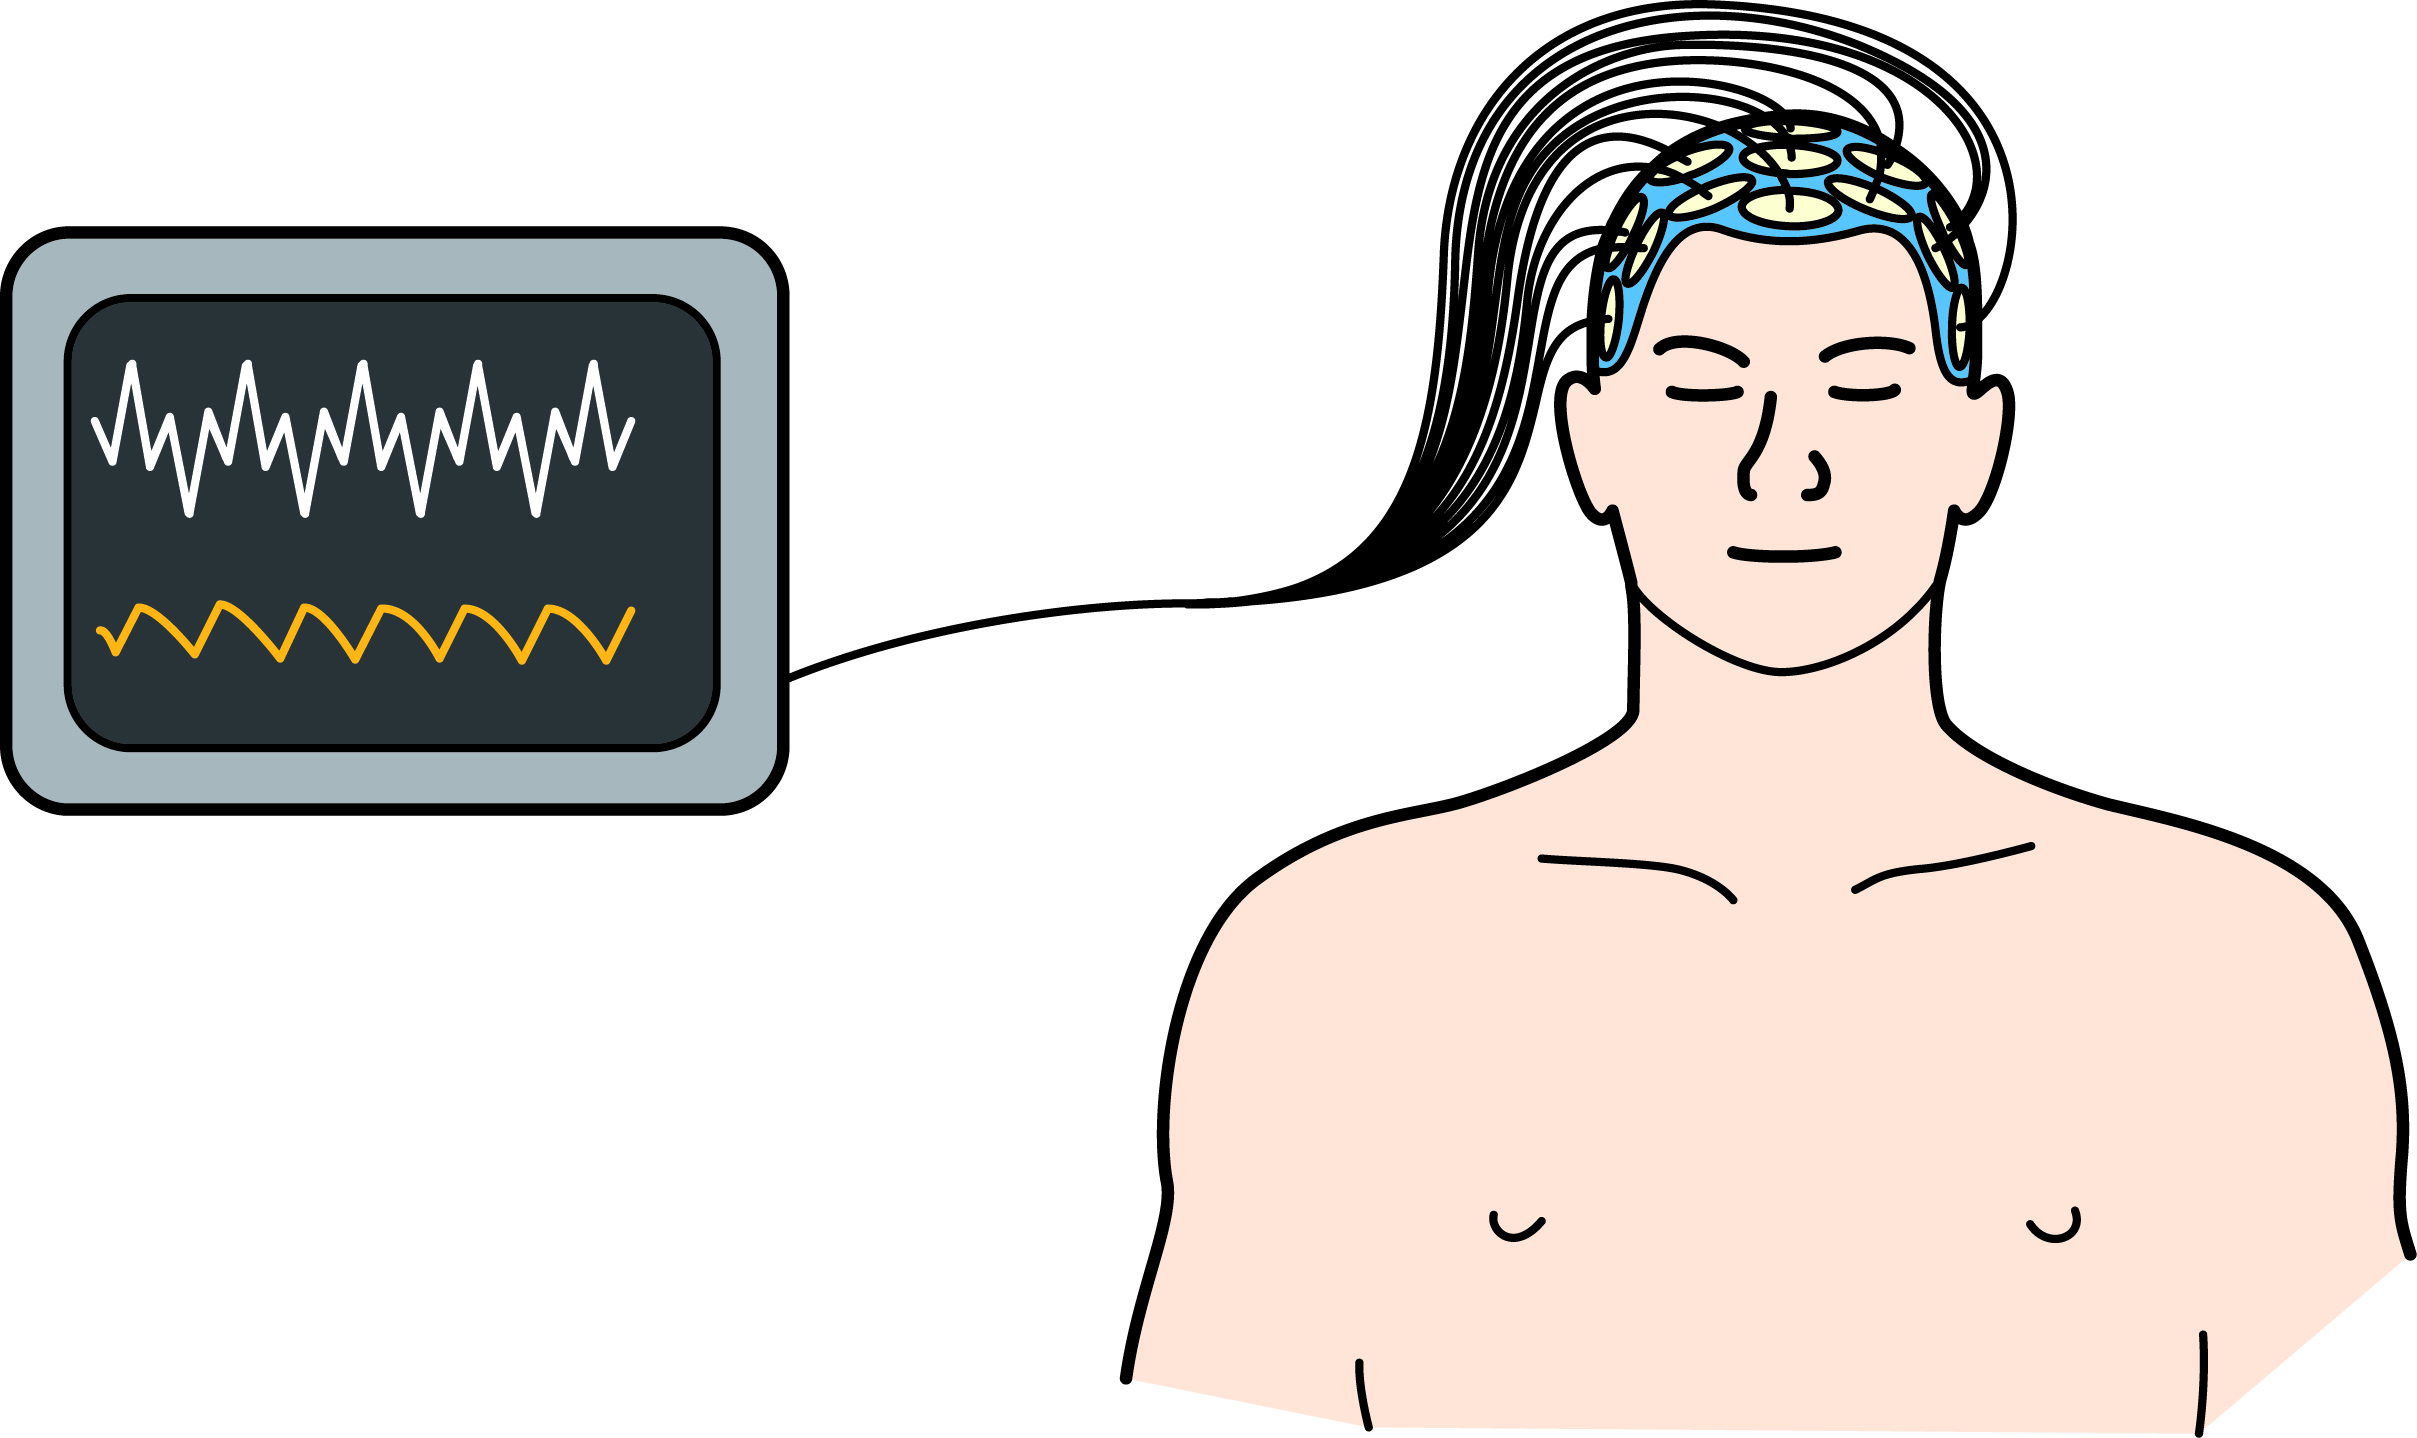
\includegraphics[width=\textwidth]{c1Introduction/eeg_easy_pics.jpg}
    \Caption{Electroencephalography (EEG) art}{\\\href{https://www.flickr.com/photos/easy-pics/9408344706}{eeg} from The Clear Communication People, licensed under \href{https://creativecommons.org/licenses/by-nc-nd/2.0/}{CC BY-NC-ND 2.0}.\\
    EEG is a form of neuroimagery with high temporal accuracy. In the noninvasive setup, a wearable cap holds electrodes in contact with the scalp. The electric potentials induced by the brain are transmitted to a digital recording system for data analysis.}
    \label{fig:c1intro:eeg}
\end{figure}

% The terms local field potentials (LFPs), electrocorticography\footnote{also termed intracranial EEG.} (ECoG) and electroencephalography (EEG) all commonly refer to measurements of electric potential: either in nerve tissue, on the directly exposed surface of the brain, or on the surface of the scalp, respectively. These types of recording apparatuses measure the summed electric activity of populations of individual cells (e.g., neurons).

For seizure monitoring and epilepsy diagnosis, video-electroencephalograms (vEEG) are the standard systems used in clinical settings. The vEEG records simultaneously videography and EEG from a particular subject, so that clinicians can observe both visual and electrophysiological epilepsy-related phenomena. EEG is also used for patient evaluation during outpatients visits, and in the ICU these sessions typically do not include video monitoring. In such cases, documentation of seizures is a challenging task which can be alleviated with seizure detection algorithms \cite{goldstein2021documentation}.

\subsection{Detecting and predicting seizures}
Computational seizure detection and forecasting with EEG data continues to be an active field of research since the 1970's \cite{mormann2007seizure, kuhlmann2018seizure}. Nonlinear methods were used in the 90's for analyzing cyclical, clustering and other time dependencies of seizure occurrences \cite{iasemidis1994time}. In the first decade of the millenium, models of EEG signals were developed to harness the dynamical processes involved in seizure generation for seizure forecasting \cite{kalitzin2005electrical}. Pattern recognition, including deep learning classifiers, have been shown to provide above chance classification in more than half of reported subjects \cite{mirowski2008comparing,mormann2016seizure}. The last two decades have seen unprecedented efforts from physicians, computer scientists and engineers to develop detective and predictive systems for epilepsy seizures \cite{jirsa2017virtual,nejedly2019deep, maimaiti2021overview}.

\subsection{Probabilistic modeling of seizure risk in epilepsy}
The global clustering and cyclical properties of epilepsy seizures has led researchers to use probabilistic models for seizure risk estimation.
% Probabilistic programming languages, which ease the Bayesian inference of complex models, have been applied to understanding seizure generation and propagation \cite{vattikonda2021identifying}.
\citet{craley2019integrating} implement a hybrid deep-learning and probabilistic-graphical-model approach and show that it outperforms baseline methods at seizure detection. A logistic regression model, tweaked with Bayes' rule to incorporate a subject-specific prior, was shown to improve forecasting in humans \cite{karoly2017circadian}. Stochastic point process models have shown promising results for integrating prior information with real-time likelihood assessments to produce forecasts of seizures hours to days in advance, although prospective clinical studies are still required to validate the applicability of these algorithms \cite{proix2021forecasting}.

\subsection{Supervised machine learning and the data labeling problem}
Prior work on automated seizure detection and prediction has focused on training machine learning models to classify EEG segments labeled as ictal, preictal or interictal. This requires expert labeling of EEG datasets for seizure events, which is both time consuming and requires extensive training. The dependence of supervised machine learning classifiers on expert-level domain knowledge makes these algorithms unsuitable for real-world forecasting devices, since expert categorical labeling solutions are still not available at scale \cite{rasheed2020machine}.
Furthermore, even clinical-grade annotations, considered to be the "gold standard" in seizure documentation, suffer from judgement bias \cite{halford2015inter}.

 \newpage
\fi

%%%%%%%%%%%%%%%%%%%%%%%%%%%%%%%%%%%%%% Chapter 2 - Deterministic Seizure Prediction %%%%%%%%%%%%%%%%%%%%%%%%%%%%%%%%%%%%%% 

\ifFULL
    \cleardoubleoddpage
    
\chapter{Pattern Recognition for Seizure Prediction}
\label{ch:2deterministic}
The field of pattern recognition includes designing pipelines to learn from data, represented as feature vectors, and recognize patterns which generalize across past and future data. A considerable amount of research has revealed that, indeed, machine learning classifiers are able to perform above-chance classification between preictal and interictal feature vectors in many patients.

Previously, the success of these methods for seizure prediction based on intracranial EEG has been demonstrated \cite{mirowski2009classification, kaggle2014contests} in human patients as well as animals. In this chapter, we show that similar results can be achieved by the same methods applied to scalp-surface EEG.


\section{Methods}
We follow closely the exploratory methods demonstrated in \citet{mirowski2009classification}. They show applications of several classifiers to seizure prediction. Bivariate feature extraction methods are used to create 2-d patterns for classification of preictal and interictal patterns (cf. figure \ref{fig:c2:nlid}).


\subsubsection{Data collection and specification}

Typical publicly available epilepsy-seizure-prediction datasets consists of long-term raw EEG recordings from pre-sugical evaluation periods, supplemented with annotations provided by approved experts \cite{handa2021open}. In these datasets, the occurrence of seizures is reported as a list of ictal (seizure) intervals
\begin{equation}
    I := \{Ictal_i\} = \{\bra{t_{start}^i|S_i|t_{end}^i} \ket{}\}
\label{eq:define_ictal}
\end{equation}
where $t_{start}$ is the seizure onset, $t_{end}$ the seizure offset, and $S_i$, when available, are the additional details reported such as epilepsy etiology, seizure type classification.
In this project, we used data from the Epilepsiae Dataset \cite{ihle2012epilepsiae}. Table \ref{table:data} lists raw recording length, sample frequency, number of surface electrodes and size-on-disk per patient.


\begin{table}[h]
\centering
% increase table row spacing, adjust to taste
\renewcommand{\arraystretch}{1.3}

% if using array.sty, it might be a good idea to tweak the value of
% \extrarowheight
\caption{Data used in this chapter.}
\label{table:data}

% % Some packages, such as MDW tools, offer better commands for making tables
% % than the plain LaTeX2e tabular which is used here.
\begin{tabular}{|c|c|c|c|c|}
\hline
\textbf{Patient Name} & \textbf{Length} & \textbf{Frequency} & \textbf{Electrodes} & \textbf{SOD} \\
\hline
\verb|pat_3500| & 92.8 h & 1024 Hz & 32 & \texttt{21 GB} \\
\hline
\verb|pat_3700| & 79.8 h & 512 Hz & 32 & \texttt{8.8 GB}\\
\hline
\verb|pat_7200| & 94.6 h & 1024 Hz & 29 & \texttt{21 GB}\\
\hline
\end{tabular}
\end{table}


\subsection{Preprocessing}
Although it is common to apply spectral filters to EEG data to reduce line noise etc., we chose to focus on the effect of classifier and features choice on predictive performance, and thus kept preprocessing to a minimum.
First, EEG channel selection was performed to select a spatially far-reaching distributed subset of 19 channels, common to all patients (see figure \ref{fig:c2det:channellocs}).



\begin{figure}[h]
    \centering
    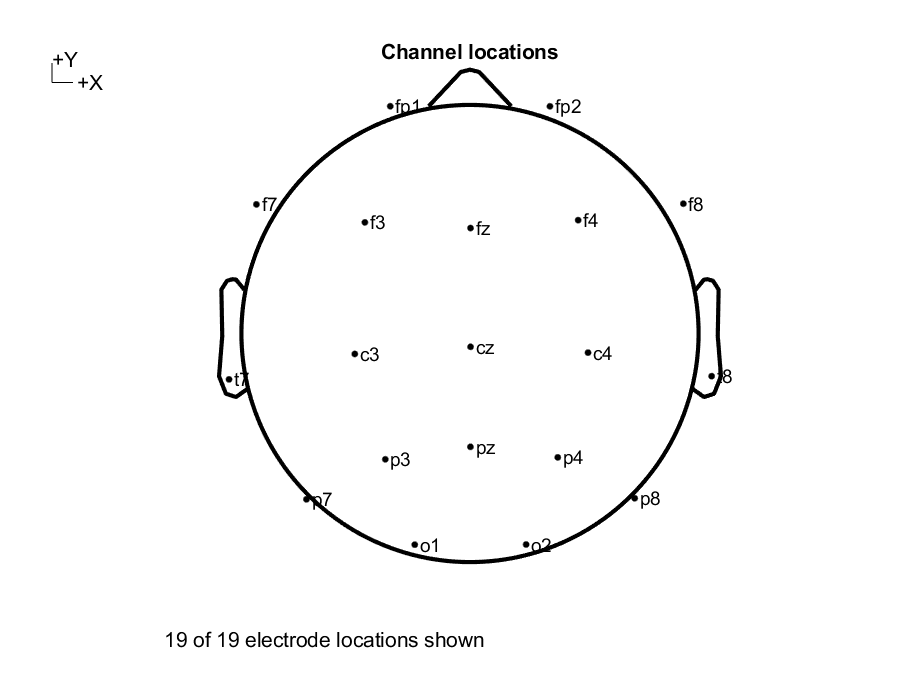
\includegraphics{c2Deterministic/Figs/PSP/topomap.eps}
    \Caption{EEG channel locations used in this chapter}{\begin{texttt}
    The common set of channels ['Fp1', 'Fp2', 'F3', 'F4', 'C3', 'C4', 'P3', 'P4', 'O1', 'O2', 'F7', 'F8', 'Fz', 'Cz', 'Pz', 'T7', 'T8', 'P7', 'P8'] was selected for all patients.
\end{texttt}.}
    \label{fig:c2det:channellocs}
\end{figure}

This was done to reduce data dimension as well as standardization amongst patients.
The raw data was resampled to 256 Hz to reduce disk space and processing time.


\subsection{Preictal and Interictal Binarization}
\label{c2:labeling}
A practical way to characterize time-varying signal dynamics is through a sliding window approach (see Fig. 1. in \cite{lehnertz2017capturing}). An EEG time series matrix $X$ is partitioned temporally into non-overlapping windows $x_1, ..., x_N$. Each window $x_i$ is given a label $y_i$, to form a dataset $D = \{(x_1, y_1),...,(x_N,y_N)\}$. Optionally, each window is transformed via a feature extraction function $f(x)$, which yields a feature-formed dataset $D_f = \{(f(x_1), y_1),...,(f(x_N),y_N)\}$.

\begin{definition}[Preictal state]
The state of preceding a seizure by a short time (minutes to hours).
\end{definition}

\begin{definition}[Interictal state]
The state of being at least a few hours before and after a seizure.
\end{definition}

Hence, each EEG window $x_i$ is checked for distance to the provided seizure labels (see eq. \ref{eq:define_ictal}) to create the appropriate label:
\begin{equation}
    y_i := 
      \begin{cases}
    0 & \text{if $preictal(x_i)$} \\
    1 & \text{if $interictal(x_i)$} \\
  \end{cases}
\end{equation}

Formally, $ictal(x_i)$ if and only if $x_i$ temporally overlaps some ictal interval $I_j$. Similarly, $preictal(x_i)$ if and only if $x_i$ overlaps with some $\tau_P$ time interval preceding an ictal interval $I_j$. Finally, $interictal(x_i)$ if and only if $x_i$ does not closely precede or proceed any seizure interval, with thresholds $\tau_{a}$ before and $\tau_{b}$ after, respectively. In this chapter, $\tau_{a}$ and $\tau_{b}$ are each taken to be 4 hours, and $\tau_P$ is taken to be 1 hour, in line with previous works and competitions such as \citet{mirowski2009classification, kaggle2014contests}.


\subsection{Bivariate Feature Extraction Methods}
\label{sec:c2:features}
The deterministic classification method relies on hand-crafted, manually engineered, features. Specifically, following \cite{mirowski2009classification}, we focus on bivariate measures of synchronicity between pairs of EEG channels (see figure \ref{fig:c2:pca_features} for examples).


\begin{figure}[htb]
    \centering
    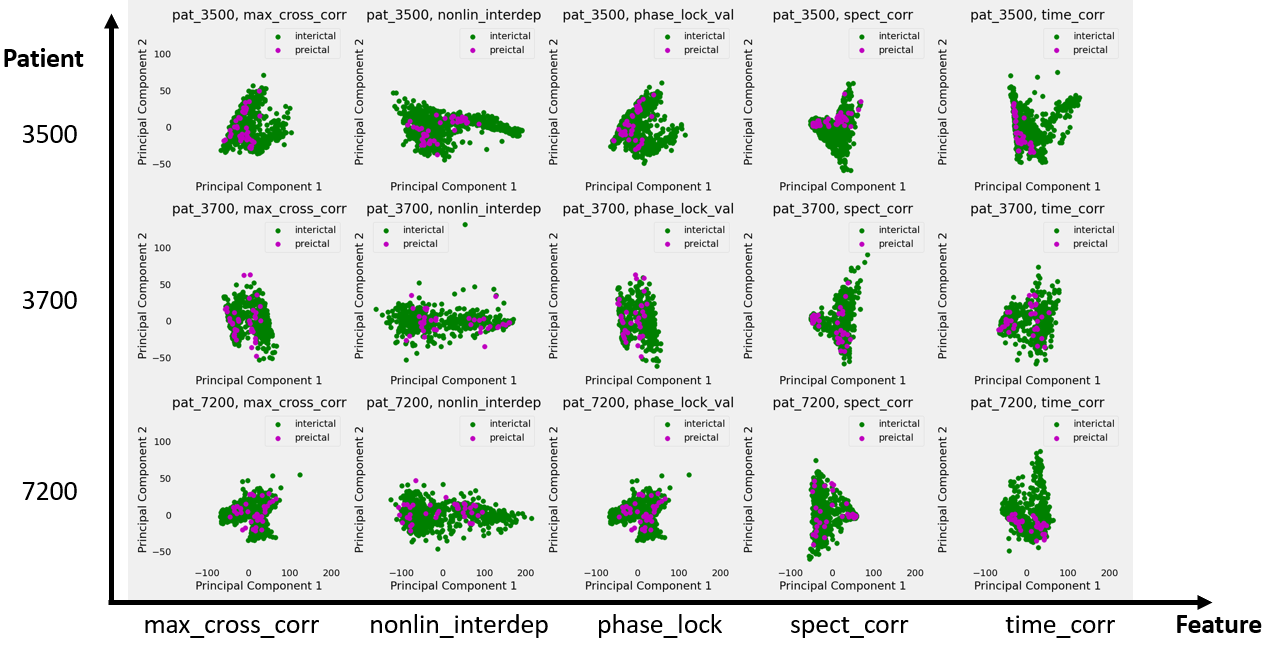
\includegraphics[width=\textwidth]{c2Deterministic/Figs/PSP/pca_features_patients2.png}
    \Caption{First 2 principal components of transformed data per patient and feature type}{The feature types are (left to right): maximal linear cross correlation, nonlinear interdependence, phase locking value, spectral domain correlation, time domain correlation. Each point represents a flattened 5-minute window (i.e., a pattern), and it's color denotes class label (interictal or preictal).}
    \label{fig:c2:pca_features}
\end{figure}

For each patient, the recording is segmented into 5 minute windows. At loading time the EEG was shifted and scaled to zero mean and unit standard deviation, per 5-minute window. Each window is segmented into 60 frames, each 5 seconds long. Each 5 second frame is reduced into a vector of length $c \cdot (c - 1) / 2$ (where $c$ is number of channels), via one of the feature extraction methods described below. Each 5 minute window is regarded a single pattern with a single label (preictal vs. interictal).


\subsubsection{Maximal Linear Cross Correlation (figure \ref{fig:c2:max_line_corr})}
In order to quantify the similarity of two signals $\{x_i\}$ and $\{y_i\}$ the maximum of a normalized cross-correlation function is taken as a measure for lag synchronization \cite{rosenblum1997phase}:

\begin{equation}
    C_{max} = \max_{\tau \in [-N,N]}{ \abs{ \frac{C_{xy}(\tau)}{\sqrt{C_{xx}(0) \cdot C_{yy}(0)} }}}
\end{equation}

Where
\begin{equation}
    C_{xy} = \begin{cases}
        \frac{1}{N-\tau}\sum_{i=1}^{N-\tau}x_{i+\tau}y_i, & \text{for } \tau >= 0\\
        C_{yx}(-\tau), & \text{for } \tau < 0
        \end{cases}
\end{equation}

is the linear cross-correlation function. $C_{max}$ is confined to the interval $[0,1]$ with high values indicating that the two signals have a similar course in time (though possibly shifted by a time lag $\tau$) while dissimilar signals will result in values close to zero.

\begin{figure}[htb]
    \centering
    \begin{subfigure}[t]{0.4\textwidth}
        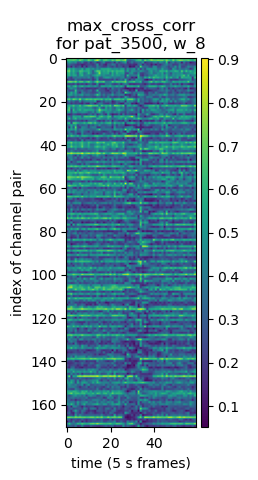
\includegraphics[width=\textwidth]{c2Deterministic/Figs/PSP/max_cross_corr.png}
        \caption{Maximal Linear Cross-Correlation}{}
        \label{fig:c2:max_line_corr}
    \end{subfigure}
    \begin{subfigure}[t]{0.4\textwidth}
    \hfill
        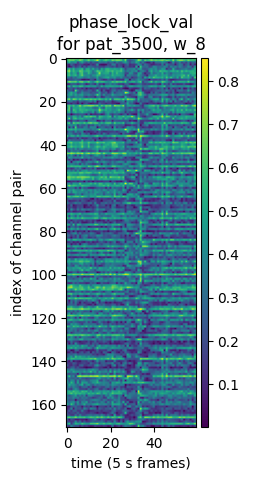
\includegraphics[width=\textwidth]{c2Deterministic/Figs/PSP/phase_lock_val.png}
        \caption{Phase Locking Value}{}
        \label{fig:c2:plv}
    \end{subfigure}
    \Caption{Two types of bivariate features}{Here are shown example patterns created by transforming 19-channel EEG recordings of length 5 minutes into maximal linear cross correlation (a) and phase locking values (b). Each row represents the feature values for a pair of channels, and each column represents those values for a particular 5 second frame. The frames are concatenated to form the window.}
    \label{fig:c2:corr}
\end{figure}



\subsubsection{Phase Locking Value (figure \ref{fig:c2:plv})}
Introduced in \cite{lachaux1999measuring}, the \emph{Phase Locking Value} measures synchronicity between eeg channels in different locations on the scalp. First, for each channel $i$, the instantaneous phase $\sigma_i ^a (t)$ of the analytical signal $x_i^a(t)$ is extracted. Then, for each pair $(i, j)$ of channels, we compute the modulus of the time averaged phase difference mapped onto the unit circle:
\begin{equation}
    PLV_{ij} = \abs{\frac{1}{T}\sum_t e^{i(\phi_i^a(t) - \phi_j^a(t))} }
\end{equation}


\subsubsection{Correlation Coefficients and Eigenvalues in the Time and Frequency Domains (figure \ref{fig:c2:corr})}
We compute the correlation coefficients between each pair of EEG channels, along with the eigenvalues of the correlation coefficients matrix, in both the time and frequency domains.
This provides two more sets of measures of synchronicity across EEG channels.

\begin{figure}[htb]
    \centering
    \begin{subfigure}[t]{0.3\textwidth}
        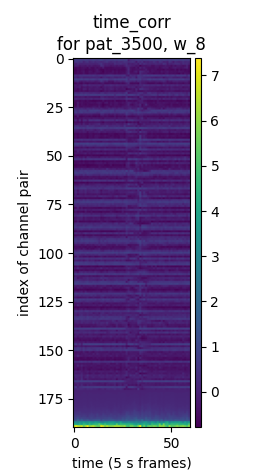
\includegraphics[width=\textwidth]{c2Deterministic/Figs/PSP/time_corr.png}
        \caption{Time-domain}{}
    \end{subfigure}
    \hfill
    \begin{subfigure}[t]{0.3\textwidth}
        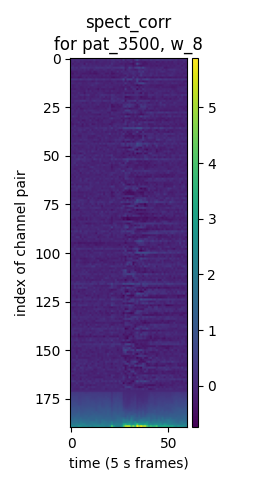
\includegraphics[width=\textwidth]{c2Deterministic/Figs/PSP/spect_corr.png}
        \caption{Spectral-domain}{}
    \end{subfigure}
    \hfill
    \begin{subfigure}[t]{0.3\textwidth}
        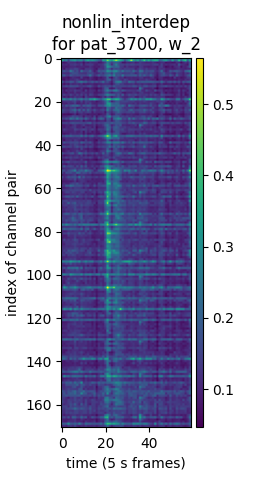
\includegraphics[width=\textwidth]{c2Deterministic/Figs/PSP/nonlin_interdep.png}
        \caption{Nonlinear Interdependence}{}
        \label{fig:c2:nlid}
    \end{subfigure}
    \Caption{Three types of bivariate features}{Example patterns created by transforming 19-channel EEG recordings of length 5 minutes into inter-channel correlation coefficients with eigenvalues appended at the bottom (a and b), and nonlinear interdependence (c).}
    \label{fig:c2:corr_and_nonlin}
\end{figure}

\subsubsection{Nonlinear Interdependence (figure \ref{fig:c2:nlid})}
The \emph{non-linear interdependence} measure for generalized  synchronization between two EEG single-channel signals $\{x_i\}$ and $\{y_i\}$ is presented in \cite{mormann2007seizure}.
First, the two signals are represented as trajectories in a state space, via time-delay embedding. Then, an asymmetric statistic measuring the Euclidean distance, in the reconstructed state-space, between trajectories  $\{\vec{x}_i\}$ and $\{\vec{y}_i\}$ is calculated for each time point. This is done for each pair of channels. See \cite{mirowski2008comparing} for more details.

\subsection{Classifiers}
We trained and tested 9 of classifiers implemented in the \emph{scikit-learn} \cite{sklearn_api} ML toolkit (v1.0.1), listed in table \ref{table:classifiers}. We chose a variety of classifiers from different families (i.e., neural networks, ensembles and decision trees).

\begin{table}[h]
\centering
% increase table row spacing, adjust to taste
\renewcommand{\arraystretch}{1.3}

% \begin{longtable}{ |c|c|c|c| }
% if using array.sty, it might be a good idea to tweak the value of
% \extrarowheight
\Caption{Classifiers used in chapter and their hyperparameter settings}{The settings chosen were the default settings provided by sci-kit learn v.1.0.1. They are repeated here for reference.}
\label{table:classifiers}

% % Some packages, such as MDW tools, offer better commands for making tables
% % than the plain LaTeX2e tabular which is used here.
\begin{tabular}{|c|c|}
\hline
\textbf{Classifier Name} & \textbf{Hyperparameters}\\
\hline
Nearest Neighbors & \texttt{K=3} \\
\hline
Linear SVM & \texttt{kernel="linear", C=0.025}\\
\hline
RBF SVM & \texttt{gamma=2, C=1}\\
\hline
Decision Tree & \verb|max_depth=5|\\
\hline
Random Forest & \verb|max_depth=5, n_estimators=10|\\
\hline
Neural Net & \verb|alpha=1, max_iter=1000|\\
\hline
AdaBoost & \verb|n_estimators=50, learning_rate=1.0, algorithm='SAMME.R'|\\
\hline
Naive Bayes & None\\
\hline
QDA & \verb|reg_param=0.0|\\
\hline
\end{tabular}
\end{table}



\section{Results}
A total of 117 classifier-datasets pairs were trained and evaluated with 5-fold cross validation, yielding a total of 585 model fits. In each fold, the classifier was trained on a random subset of 80\% of the data, and tested on the remaining 20\%.


\subsection{Evaluation Metrics}
We report the following metrics for all features-classifiers pairs:
\begin{enumerate}
    \item ROC AUC
    \item Precision
    \item Recall
    \item fit time
    \item score time
\end{enumerate} 


\subsection{Classifier and Feature Comparison}
Figures \ref{fig:c2:mean_roc_auc} and \ref{fig:c2:std_roc_auc} show the mean and standard-deviation for each classifier on each feature set, for each patient. It is found that the Linear SVM and Neural Net (MLPClassifier) are the top two performers consistently, sometimes followed closely by the Nearest Neighbor Classifier.


\begin{figure}[!htb]
    \centering
    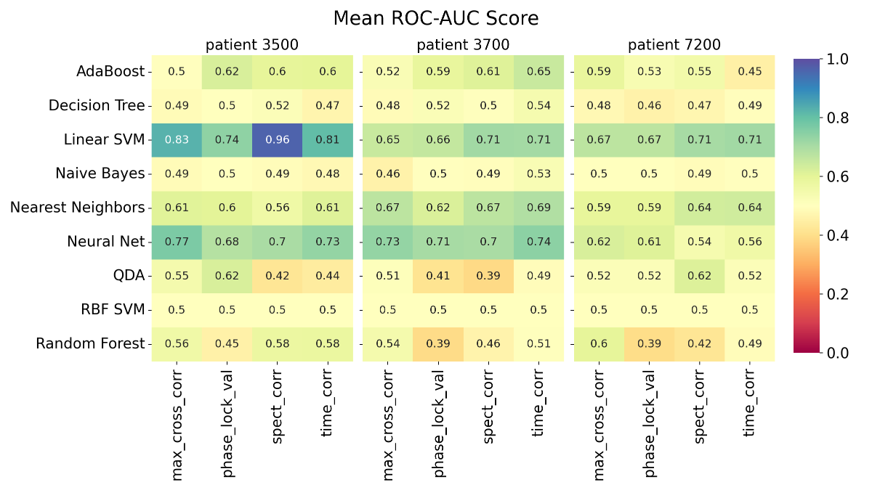
\includegraphics[width=\textwidth]{c2Deterministic/Figs/PSP/mean_roc_auc_classifiers_and_features.png}
    \Caption{Mean AUC-ROC scores for 5-fold cross validation.}{}
    \label{fig:c2:mean_roc_auc}

    \centering
    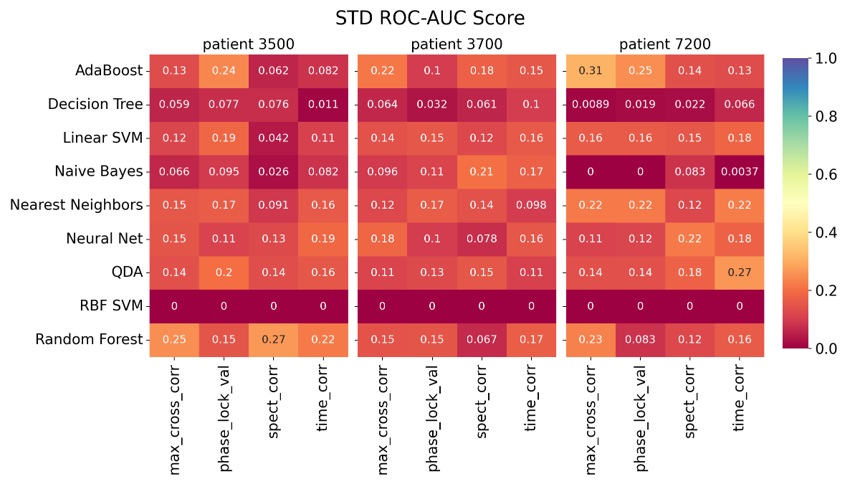
\includegraphics[width=\textwidth]{c2Deterministic/Figs/PSP/std_roc_auc_classifiers_and_features.png}
    \Caption{Standard deviation of AUC-ROC scores for 5-fold cross validation.}{}
    \label{fig:c2:std_roc_auc}
\end{figure}


\subsection{Training Efficiency}
Figure \ref{fig:c2:training_times} shows the mean time it took to fit each classifier to each feature-set, for each patient, over 5-fold CV. It is shown that the neural network, ensemble method (AdaBoost) and support-vector-machines consistently take longer than the decision tree, naive-Bayes, quadratic discriminant analysis, and random forest classifiers.

\begin{figure}[tb]
    \centering
    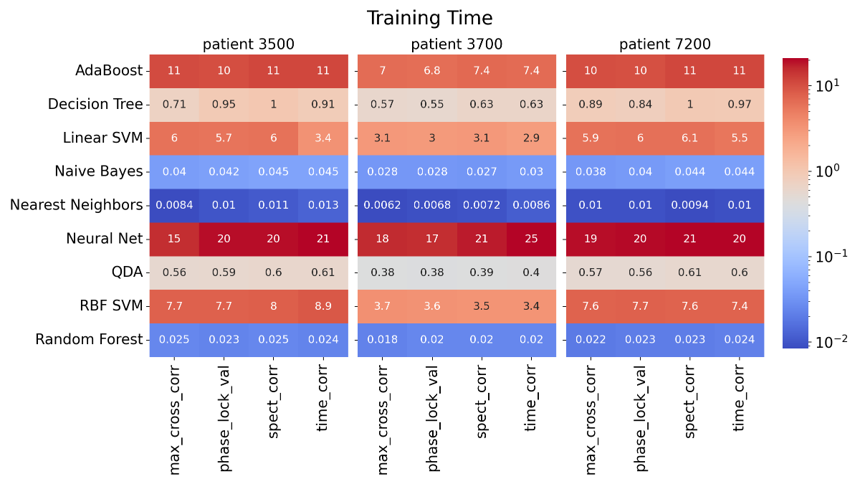
\includegraphics[width=\textwidth]{c2Deterministic/Figs/PSP/training_time_classifiers_and_features.png}
    \Caption{Mean training times (in seconds) for fitting the classifiers to the datasets.}{}
    \label{fig:c2:training_times}
\end{figure}

\subsection{Comparing Feature Sets}
The Linear SVM, which performed best in the previous experiments, is selected to compared the predictive performance of the different feature types. Notably, the classifier performed above chance in all feature sets, with the spectral correlation coefficients features slightly outperforming the others with respect to the ROC AUC score. See figures \cref{fig:c2det:350_svm,fig:c2det:370_svm,fig:c2det:720_svm}.

\begin{figure}[htp]
    \centering
    \subfloat[patient 3500]{%
      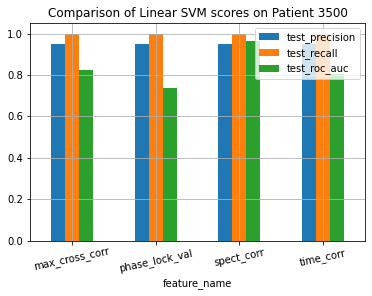
\includegraphics[clip,height=0.3\textheight]{c2Deterministic/Figs/PSP/pat_350_svm_features.png}
      \label{fig:c2det:350_svm}
    }

    \subfloat[patient 3700]{%
      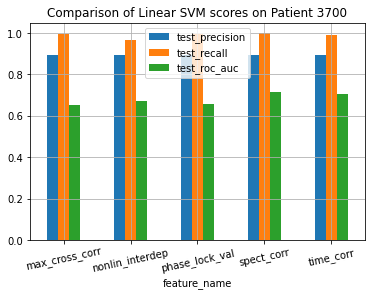
\includegraphics[clip,height=0.3\textheight]{c2Deterministic/Figs/PSP/pat_370_svm_features.png}
    \label{fig:c2det:370_svm}
    }

    \subfloat[patient 7200]{%
      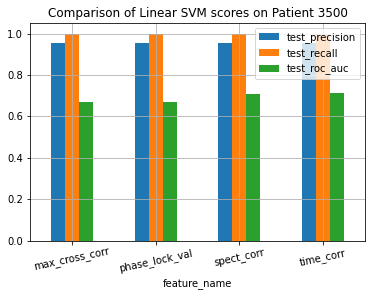
\includegraphics[clip,height=0.3\textheight]{c2Deterministic/Figs/PSP/pat_720_svm_features.png}
    \label{fig:c2det:720_svm}
    }

    \Caption{Results of Linear SVM on different feature datasets}{}

    % \begin{subfigure}[t]{}
    % \centering
    % 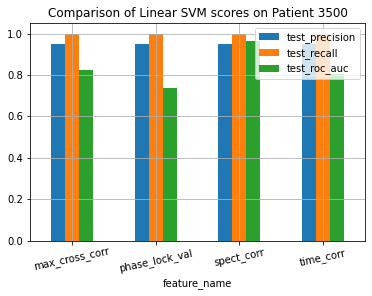
\includegraphics[height=0.3\textheight]{c2Deterministic/Figs/PSP/pat_350_svm_features.png}
    % \Caption{Comparison of predictive performance of Linear SVM for Patient 3500 on different feature datasets}{}
    % \label{fig:350_svm}
    % \end{subfigure}
    
    % \vfill
    % \begin{subfigure}[t]{}
    % 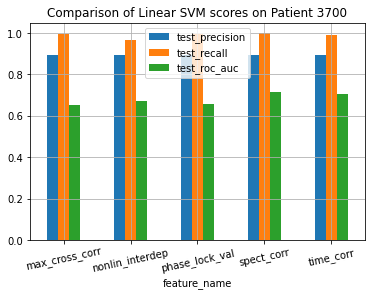
\includegraphics[height=0.3\textheight]{c2Deterministic/Figs/PSP/pat_370_svm_features.png}
    % \Caption{Comparison of predictive performance of Linear SVM for Patient 3700 on different feature datasets}{}
    % \label{fig:370_svm}

    % \end{subfigure}
    
    % \vfill
    
    % \begin{subfigure}[t]{}
    % 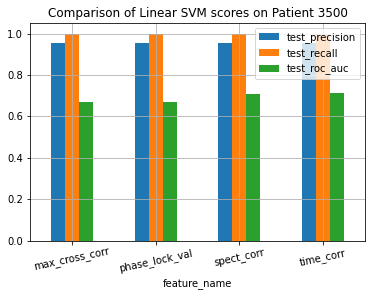
\includegraphics[height=0.3\textheight]{c2Deterministic/Figs/PSP/pat_720_svm_features.png}
    % \Caption{Comparison of predictive performance of Linear SVM for Patient 7200 on different feature datasets}{}
    % \label{fig:720_svm}
    % \end{subfigure}
    
\end{figure}


\section{Conclusion \& Discussion}

In this chapter, we explore the pattern recognition approach in a similar fashion to \citet{mirowski2009classification}, albeit on a newer dataset of noninvasive, 19 channel surface-EEG. We achieve comparable results across 3 subjects, with ROC-AUC scores commonly between 0.7-0.8 for a variety of bivariate feature sets related to inter-channel synchronicity with support vector machines.


\Citet{mirowski2009classification} evaluated their pipeline on 6-channel, intracranial data from 21 epilepsy patients. In this chapter, we use 19-channel data from surface EEG, from 3 patients. They reported 71\% sensitivity with 0 false alarms, on 15 out of the 21 patients they assessed. We trained 117 classifiers in different combinations of classifier-dataset. On the best classifier for each patient, only Patient 3700 achieves over 70\% sensitivity at the 0 false alarms threshold. For Patients 3500 and 7200, the sensitivities at 0 false alarms are 42\% and 40\%, respectively.

The main contribution of this chapter is to show that the classification of synchronicity-based features for seizure prediction is possible not just with intracranial data as in \cite{mirowski2009classification}, but also with surface-EEG from \citet{ihle2012epilepsiae}. Another difference between our data and the data analyzed in the previous work is the number of EEG-channels. Although the increase from 6 (15 pairs) to 19 (171 pairs) EEG channels gives us more sources of information, it also leads to a larger sample space such that probably much more data is needed.

This chapter showcases the predictive power of different classifiers and synchronicity-based features applied to noninvasive EEG data. We trained various classifiers. While some classifiers failed to generalize at all, most classifiers were successful in classifying better than chance, with AUC-ROCs in the range 0.67-0.81 commonly achieved. When comparing the synchronicity features, we did not find any of the feature sets to be remarkably better than the others in any of the 3 patients. 


% \begin{figure}[h]
%     \centering
%     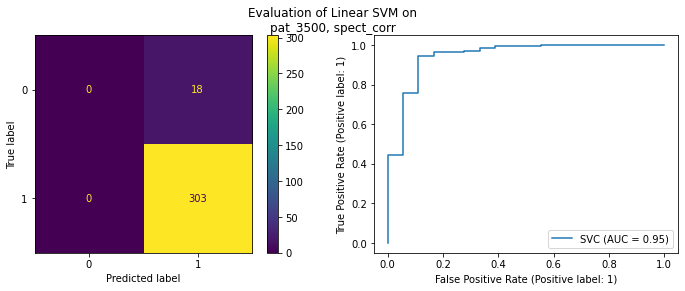
\includegraphics[width=\textwidth]{c2Deterministic/Figs/PSP/pat_350_best.png}
%     \caption{Plot of Confusion Matrix and ROC Curve for the highest scoring classifier for Patient 3500}
%     \label{fig:350_best}
% \end{figure}

% \begin{figure}[h]
%     \centering
%     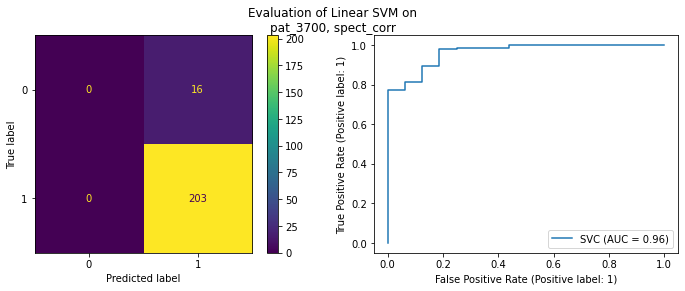
\includegraphics[width=\textwidth]{c2Deterministic/Figs/PSP/pat_370_best.png}
%     \caption{Plot of Confusion Matrix and ROC Curve for the highest scoring classifier for Patient 3700}
%     \label{fig:370_best}
% \end{figure}

% \begin{figure}[h]
%     \centering
%     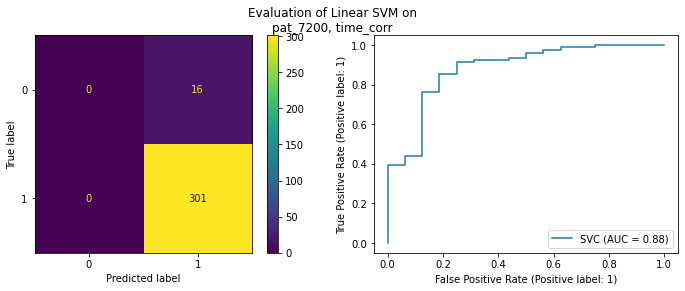
\includegraphics[width=\textwidth]{c2Deterministic/Figs/PSP/pat_720_best.png}
%     \caption{Plot of Confusion Matrix and ROC Curve for the highest scoring classifier for Patient 7200}
%     \label{fig:720_best}
% \end{figure}



% \newpage
 \newpage
\fi

%%%%%%%%%%%%%%%%%%%%%%%%%%%%%%%%%%%%%% Chapter 3 - Bsle %%%%%%%%%%%%%%%%%%%%%%%%%%%%%%%%%%%%%% 

\ifFULL
    \cleardoubleoddpage
    
%%%%%%%%%%%%%%%%%%%%%%%%%%
\chapter{Bayesian Estimation of Seizure Likelihood}
\label{ch:3Bsle}

The recently reported paradigm shift from binary classifications to probabilistic forecasts of seizure risk has been illustrated conceptually in recent works such as \shortcites{karoly2017circadian, baud2018multi}\citet{karoly2017circadian, baud2018multi, baud2020chance}. They discuss the need to consider \emph{pro-ictal} states - states to which we attribute a higher seizure likelihood, that does not necessarily result in a seizure. The likelihood is based on a priori knowledge or assumptions.

In our work, we propose a Bayesian inference based algorithm, namely Bayesian Seizure Likelihood Estimation (BSLE)\footnote{code can be found at \url{https://github.com/noamsgl/msc}.}, and evaluate it on intracranial EEG from canines with epilepsy. It is different than the previously mentioned works by estimating the likelihood in an unsupervised way, dismissing the need for accurate seizure event labels.

%%%%%%%%%%%%%%%%%%%%%%%%%%%%%%%%%%%%%%%%%%%%%%%%%%%%%%%%%%%%%%%%%%%%%%%%%%%%%%%%%%%%%%%%%%%%%%%%%%%%%%%%

\section{Background}
The purpose of this section is to introduce preliminary concepts necessary to understand the probabilistic approach.

% Lower the section header to match the (very) long chapter header
% \renewcommand*\sectionmarkformat{\\ \autodot\thesection\enskip}
%%%%%%%%%%%%%%%%%%%%%%%%%%


% \renewcommand*\sectionmarkformat{\autodot\thesection\enskip}
%%%%%%%%%%%%%%%%%%%%%%%%%%
\subsection{Problem description}
\label{sec:2background:setup}

There is a continuous EEG recording system sampling at $f$ Hz (see figure \ref{fig:c3bsle:caninedb}). We are provided with a dataset $D = \{e_t, a_t\}_{t_0}^{t_m}$. For each time $t$, $e_t \in \mathbb{R}^{c \times f \cdot T}$ is the observed EEG segment with $c$-channels of duration $T$, ending at time $t$. Also, $a_t \in \{0, 1\}$ is a clinically-approved seizure annotation corresponding to the observed interval $[t - T, t]$. The annotation denotes the expert's best judgement as to whether a seizure event began within the corresponding time-window.

The problem at hand is to find a forecaster $f_\tau^*$ with 
predictive qualities of interest. First, a general definition of seizure forecasting is provided. This setup is made more specific in the evaluation section (\ref{sec:c3bsle:results}).

\begin{definition}[seizure forecaster with horizon $\tau$]
    a function of the form $$ \hat{s}_{t+\tau} = f_\tau(e_t, a_{0:t})$$ where $s_{t+\tau}$ is the seizure risk in the interval $[t, t+\tau]$,  $e_t$ is the current EEG observation, $a_{0:t}$ is the past event history, and $\tau$ is the forecast horizon. The horizon parameter $\tau$ can take negative values, to mean detecting seizure events post-observation.
\end{definition}

\begin{figure}[p]
    \centering
    \includegraphics[width=\textwidth]{c3Bsle/Figs/canine/MayoClinic_CanineEpilepsy_print.pdf}
    \Caption{Data collection and required output}{From \citet{coles2013feasibility}. Used with permission of Mayo Foundation for Medical Education and Research, all rights reserved.\vspace{3mm}\\ The Canine-Epilepsy dataset was used for empirical evaluation in this chapter, chosen primarily because it is publicly available and the per-subject recording length is long. The EEG is collected and processed by a forecasting algorithm to produce a seizure risk gauge (bottom).}
    \label{fig:c3bsle:caninedb}
\end{figure}
\clearpage

\subsection{Probabilistic representation of EEG and seizures in time}
\label{sec:c3Bsle:model}

We capture the notion of EEG observations and seizure events by random variables (r.v.s):

\begin{align}
	 e_t \sim E(t) &\in \Omega_E = \mathbb{R}^{c \times N}\\
	 s_t \sim S(t) &\in \Omega_S = \{0, 1\}
\end{align}

where $\Omega_{E}$ ($\Omega_{S}$) is the sample space for the r.v. $E$ (the r.v. $S$). $c$ is the number of EEG-channels, $N$ is the number of samples recorded (\aka segment length) over a duration $T$. We define the event that a seizure began within $[t-T, t]$ as $\{S(t) = 1\}$ (see figure \ref{fig:c3bsle:sample_space}). 

\begin{figure}[!ht]
    \centering
    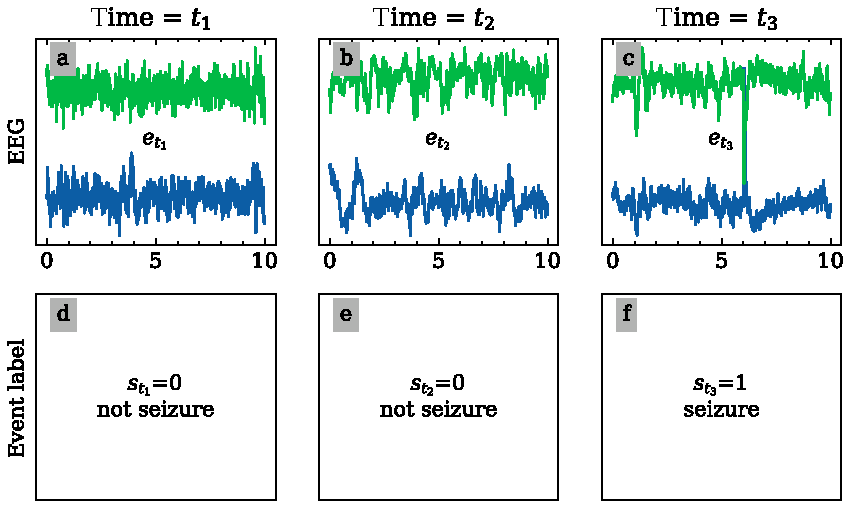
\includegraphics{c3Bsle/Figs/intro/sample_space.pdf}
    \Caption{Sample space $\Omega_E \times \Omega_S$}{In the probabilistic model, EEG segments and seizures are plausible events. For example, a 2-channel 400 $Hz$ EEG segment of length 10 seconds is a realization of the random variable E 
    supported by $\mathbb{R}^{2 \times 400}$. Likewise, the occurrence of a seizure at time $t_i$ is denoted by $s_{t_i} = 1$ as opposed to $s_{t_i} = 0$.}
    \label{fig:c3bsle:sample_space}
\end{figure}



\section{Model specification}
Formally, the proposed model is a multilevel probabilistic model, as shown in figure \ref{fig:c3bsle:bsle_net_intro}. To overcome the curse of dimensionality, first the raw time signal is embedded in a low dimensional manifold. Then, Bayesian inference is applied with custom evidence, prior and likelihood functions to infer the probability $\prob(s_t \mid e_t)$.

% Representing a typical 10-second EEG segment requires about \num{6.4e4} scalar values in it's raw form, thus special care is taken to overcome the curse of dimensionality. 

% partial Bayesian Seizure Annotation Model
\begin{figure}[htbp]

  \tikz{

    % nodes
     \node[obs] (e) {$e_{t}$};%
     \node[latent, above=of e, xshift=1cm] (s) {$s_{t}$}; %
    \node[obs, below=of s, xshift=1cm] (a) {$a_{t}$};%

    % gates

    % edges
     \edge {s} {e, a}

    % plates
    \plate[inner sep=10pt] {plate1} {(e)(a)(s)} {time $t$}; %

    % text
     \node[text width=6cm, anchor=west, right] at (4,1)
     {
       \begin{alignat*}{3}
        e_t & \mid s_t \sim \mathcal{D}_{E \mid S} && \text{ // EEG embeddings conditioned on seizure variable}\\
        a_t & \mid s_t \sim \mathcal{D}_{A \mid S} && \text{ // Annotation conditioned on seizure variable}\\
       \end{alignat*}
     };
   }
 \Caption{Probabilistically Modeling Seizure Occurrence, EEG signal and Annotations across Time}{The nodes represent random variables. The shaded nodes $e$ and $a$ represent the observed variables EEG and Annotations, respectively. The $s$ node represents a latent variable, whose values can be inferred with Bayes' theorem. The }
  \label{fig:c3bsle:bsle_net_intro}
\end{figure}

\subsection{EEG embedding}
\label{sec:c3bsle:embedding}
A Gaussian process (GP) is a mathematical entity often used in Bayesian time series modeling. It allows flexible modeling of smoothness, periodicity and other interpretable signal properties. Existing algorithms which perform posterior inference over the underlying hyperparameters are available \cite{rasmussen2003gaussian, gardner2018gpytorch}. We embed the EEG data in the low-dimensional manifold of GP hyperparameters (see figure \ref{fig:c3bsle:embeddings}). These hyperparameter values are then used to represent the EEG in the following procedures. Technical details of the embedding process are provided in appendix \ref{apx:GPEmbed}.

\begin{figure}[h]
      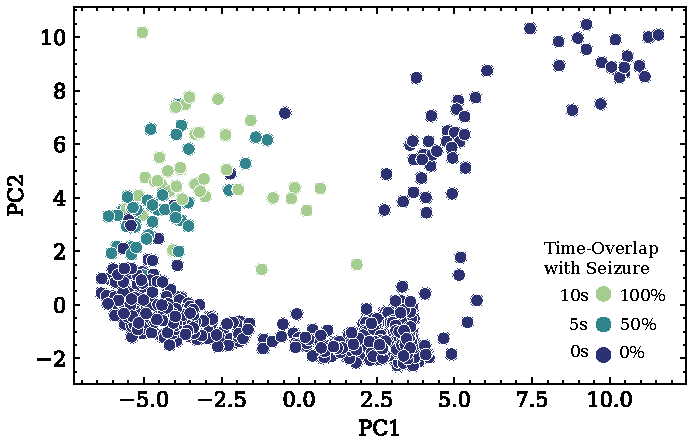
\includegraphics[width=\textwidth]{c3Bsle/Figs/embeddings/embeddings_double.pdf}
      \Caption{EEG embedding in Gaussian process hyperparameter space}{Each point represents a 10-second EEG segment fit with a Gaussian process, and displays the first two principal components of the hyperparameters vector. The color indicates the time of the recording relative to the seizure annotations. The ictal embeddings are found to be distinguishable from the interictal embeddings in the space of GP-hyperparameters.}
      \label{fig:c3bsle:embeddings}
\end{figure}


\subsection{Bayesian estimation}
We wish to construct a model for $\prob[S, E, t]$, and then apply it with Bayes' rule to infer the likelihood of a seizure at time $t$ determined by an EEG recording:

\begin{equation}
\texttt{probability}[\texttt{seizure=}S \mid \texttt{time=}t, \texttt{EEG=}E] \propto \prob[E \mid S, t] \prob[S \mid t]
\end{equation}

It should be evident that this procedure is general in that each component on the right-hand-side can be estimated independently, and then combined via multiplication.

In the case of epilepsy, handling uncertainty in the face of evidence plays a major role, thus naturally appealing to the mathematical machinery termed Bayes' theorem.

We apply Bayes' theorem to estimate the updated likelihood of a seizure after observing an EEG signal:

% \begin{align}
%     \underset{posterior}{\prob(S \mid E)} = \frac{\prob(E \mid S) \prob(S)}{\prob(E)} \propto \underset{likelihood}{\prob(E \mid S)} \cdot \underset{prior}{\prob(S)}
% \end{align}


\begin{align}
    \underset{posterior}{\prob(S \mid E)} = \frac{\underset{likelihood}{\prob(E \mid S)} \underset{prior}{\prob(S)}}{\underset{evidence}{\prob(E)} } 
\end{align}


For bayesian inference, the likelihood, prior and evidence functions need to be defined and approximated. We now derive the mathematical formulations for each of these, which should complete the description of our inference procedure.


\subsubsection{Likelihood Definition}
For a patient with epilepsy, we hypothesize that the anomalies in EEG data are inherently more likely to reflect underlying seizure events, because seizures are rare events. First, we define an unsupervised density-quantile novelty score. Then, we establish the seizure likelihood function by adding a threshold parameter.

\paragraph{Density estimation}
A Gaussian mixture model (GMM) with 4 components and full inter-component covariance matrix is fit to the data in GP-hyperparameter space, to give a density estimation:

\begin{definition}{Density estimation}
    $\hat{p}(e) \approx pdf(E)$
\end{definition}
\label{eq:c3bsle:de}

Mathematical details are provided in appendix \ref{apx:GMM}. See figure \ref{fig:3bsle:de}.

\begin{figure}[hp]
    \centering
    \begin{subfigure}[h]{\floatwidth}
        \showthe\textwidth
          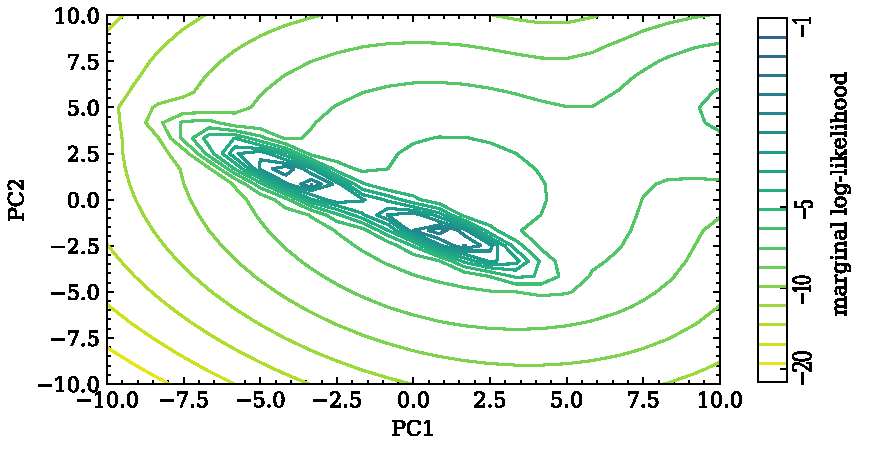
\includegraphics[width=\textwidth]{c3Bsle/Figs/densityestimation/de_pc1_pc2.pdf}
          \caption{First and second principal components}
    \end{subfigure}
  	\begin{subfigure}[h]{\floatwidth}
  	    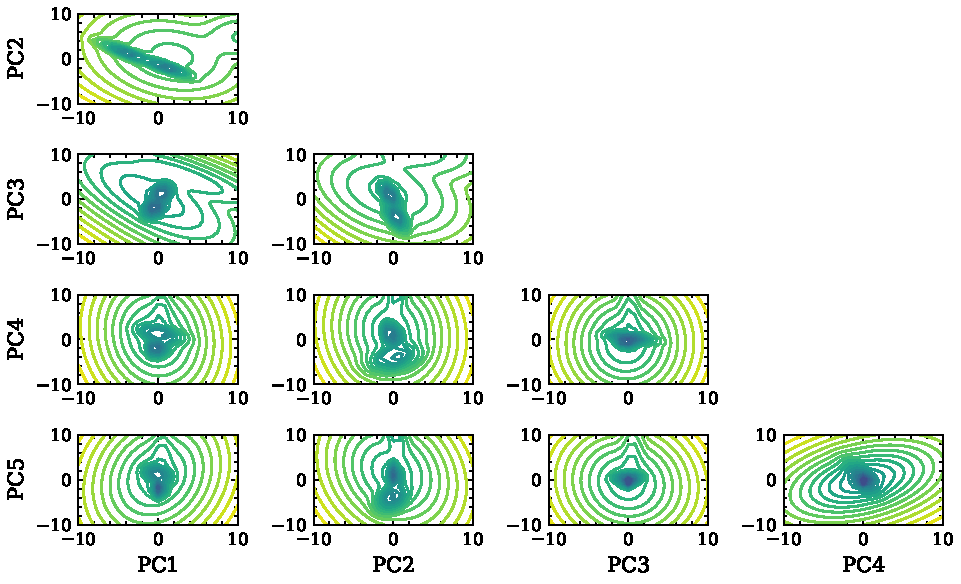
\includegraphics[width=\textwidth]{c3Bsle/Figs/densityestimation/de_pc_pair_plot.pdf}
  	    \caption{Pair plots for the first five principal components}
  	\end{subfigure}
    \Caption{Contour plots for multidimensional density estimation}{An estimator $\hat{p}(e_t)$ is computed using a GMM with 4 components fit to the first 5 principal components of the data as represented by GP hyperparameters. The contour plot of $\log \hat{p}(e_t)$ is shown for every pair of principal components by marginalizing 
    over the remaining axes. The regions with lower likelihood are more likely to be classified as seizures.}
    \label{fig:3bsle:de}
\end{figure}



\paragraph{Density quantile approach to Novelty Scores}

A Monte Carlo technique, namely the Density Quantile Approach, is used to obtain information about the probability coverage of a given region of the sample space. Given a new sample $e$, the novelty score is the quantile (also known as a $p_{value}$) of $\hat{p}(e)$ relative to the random variable $E$, as approximated by a sample dataset $D$. This calculation has been shown to converge tractably to the probability density function quantile as the sample size grows \cite{hyndman1996computing}. 

\begin{definition}{Novelty Score}
    \begin{equation}
    \label{eq:c3bsle:novelty_score}
    \mathcal{Z}(e^{new}) = \frac{\left|\{ e_i \mid \hat{p}(e^{new}) \le \hat{p}(e_i) \} \right|}{|\{ e_i\} |}
    \end{equation}
\end{definition}

The essence of the novelty score $\mathcal{Z}(e^{new})$ is that it maps data samples to the interval $[0, 1]$, such that more anomalous samples (i.e. samples from less dense regions) are given larger values.

In accordance with our rarity of seizures hypothesis, a new normal (nonseizure) EEG observation $e^{new}$ will be relatively similar to previously seen observations in $\{ e_i \}$, leading to a low novelty score. Conversely, for abnormal (seizure) data, the data will be relatively dissimilar, leading to a high novelty score.

In order to utilize this hypothesis in the BSLE likelihood function, we flip the sign of the $S$ parameter to $\neg S$ meaning not a seizure, thus modeling $\prob(E \mid \neg S)$ directly.

\paragraph{Partitioning with a threshold $\alpha$}
A new threshold parameter $\alpha$ is introduced to guide the BSLE likelihood function $P(E \mid \neg S ; \alpha)$. Using the density estimator $\hat{p}(e)$, we partition the GP-hyperparameter sample space $\Omega_{GP}$ into a low density region and a high-density region, and treat each region differently. The threshold parameter $\alpha$ affects the location of the region split.

\begin{definition}[$\alpha$-Highest Density Region]
    Let $f(x)$ be the density function of a random variable $X$. Then the $100(1-\alpha)\%$ HDR is the subset $R(f_\alpha)$ of the sample space of $X$ such that
    $$R(f_\alpha) = \{ x : f(x) \ge f_\alpha \}$$
    where $f_\alpha$ is the largest constant such that $\prob(X \in R(f_\alpha)) \ge 1-\alpha$.
\end{definition}
 
\begin{definition}[BSLE likelihood]

% \prob\!\left(E \middle\vert \neg S\right) 
\begin{equation}
\label{eq:c3bsle:likelihood}
\prob(e^{new} \mid \neg S ; \alpha) = \begin{cases}
\mathcal{Z}(e^{new}) &\text{if $e^{new} \in HDR_\alpha$}\\
0 &\text{if $e^{new} \notin HDR_\alpha$}
\end{cases}
\end{equation}

Intuitively, the $\alpha$ parameter determines the interplay between auto-rejection of a sample and estimation of its seizure likelihood. 
\end{definition}



\subsubsection{Evidence Definition}
\begin{definition}[BSLE Evidence]
    \begin{equation}
    \label{eq:c3bsle:evidence}
    \prob(E) = \prob(\{pdf(e) \leq pdf(E)\})
    \end{equation}
\end{definition}


\subsubsection{Prior definition}
The prior function is where the Bayesian modeler induces intentional bias into the inference process. We define and compare two priors, to show that our model is general in this respect.

\paragraph{Weakly supervised cyclical prior}
This prior encourages forecasters to inhibit a circadian - twenty four hour long - cyclical preference. We construct mathematically the cyclical prior as a linear mixture of 24 circular Gaussian distribution kernels, as in \cite{karoly2017circadian}.

% circular Gaussian distribution definition
\begin{definition}[Circular Gaussian Distribution]
    % $$ \hat{y}_{t+\tau} = f(e_{t-k:t}, a_{0:t})$$
    \begin{align}
    f(x | \mu, \kappa ; \omega) = \frac{\exp (\kappa \cos (\omega (x - \mu)))}{2 \pi I_0(\kappa)}
    \label{eq:2background:vm_density}
\end{align}

In this work, we set $\omega \gets \frac{2\pi}{24}$ to scale the period to 24-hours, and drop it from the notation for brevity in the following text.

% \begin{figure}
%     \centering
%     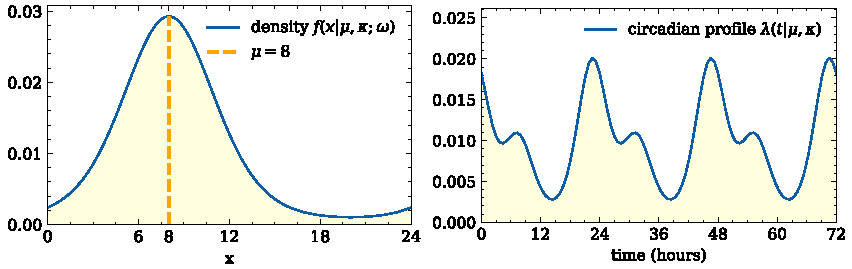
\includegraphics{c3Bsle/Figs/model/vm_and_circadian_profile.pdf}
%     \caption{Caption}
%     \label{fig:my_label}
% \end{figure}
\label{def:circ_gaussian}
\end{definition}


\begin{figure}[h]
    \centering
    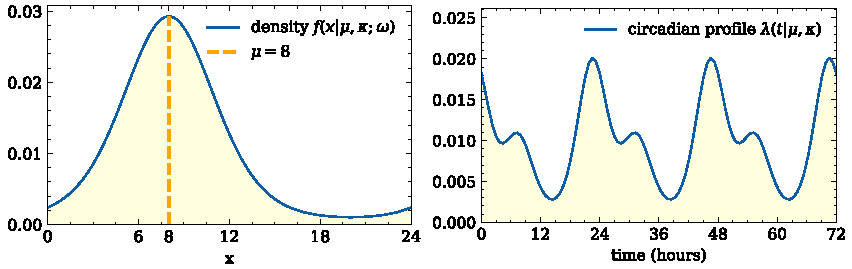
\includegraphics{c3Bsle/Figs/model/vm_and_circadian_profile.pdf}
    \Caption{Circular Gaussian (von Mises) distribution and circadian profile}{
The circular Gaussian distribution is similar to a bell-shaped normal distribution on a circle (left).\\A mixture of von Mises distributions represents the cyclical seizure base-rate behavior, termed \emph{circadian profile} (right).}
    \label{fig:c3bsle:vm}
\end{figure}

% uniform prior definition
\begin{definition}[Circadian prior]
    \begin{equation}
    \label{eq:c3bsle:cyclical_prior}
    \prob(S_t) = \frac{1}{K}\sum_{i=0}^{23} f(t \mid i, k)
    \end{equation}
    where $K$ is a normalizing constant evaluated numerically (\texttt{np.trapz}).
\end{definition}

\begin{figure}[h]
    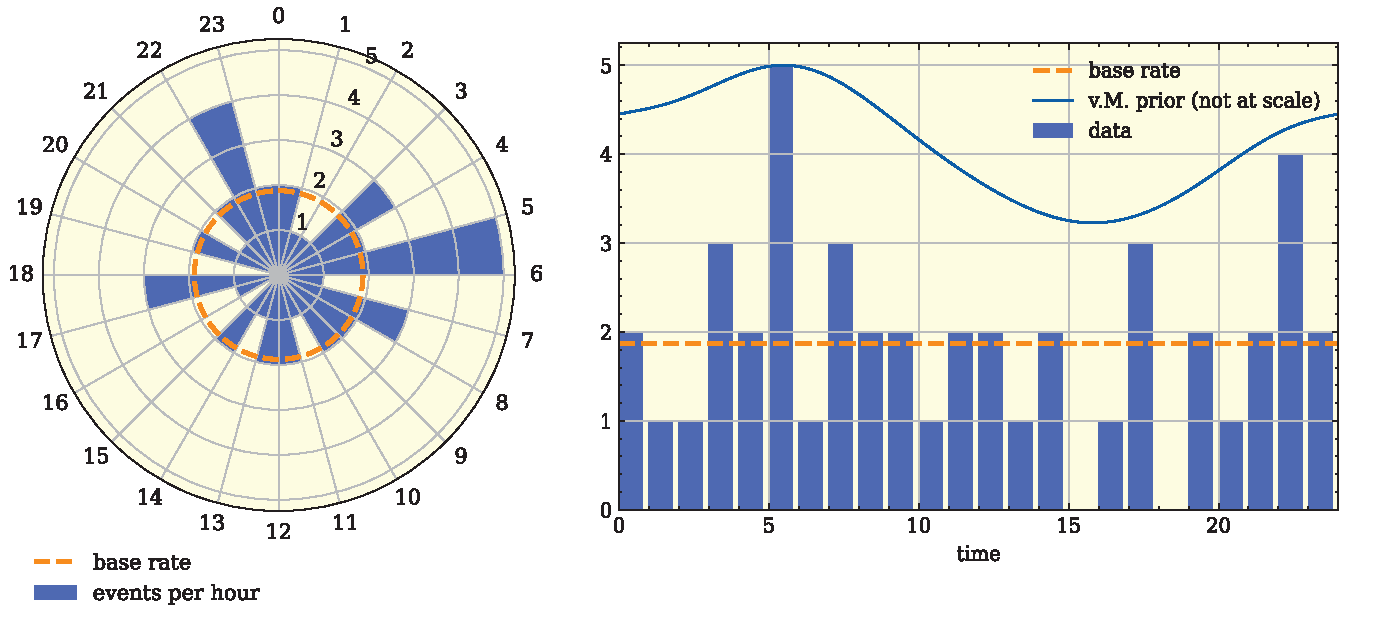
\includegraphics[width=\textwidth]{c3Bsle/Figs/prior/vm_prior_histogram.pdf}
    \Caption{Circadian Seizure Histogram and Circadian Profile}{The 45 seizure events of canine \texttt{I004\_A0003\_D001} from 465 days are binned by hour-of-the-day into a polar histogram (left). A von Mises mixture density function, with kernel weights given by the circadian histogram, is plotted (right).}
    \label{fig:c3bsle:circadian_hist_vm}
\end{figure}

% uniform prior definition
\begin{definition}[Uniform prior]
The uniform prior takes a constant value for all time points: 
    \begin{equation}
    \label{eq:c3bsle:uniform_prior}
    \prob(S_t) = \lambda_0 \cdot T
    \end{equation}
    where $\lambda_0$ is a constant seizure rate, and $T$ is the observation duration.
    Without loss of generality, we set $\lambda_0 = \frac{1}{10 \text{ day}}, T = 10 \text{ sec}$.
\end{definition}
This prior issues equal seizure plausibility to all time points, nullifying the time covariate's effect on the seizure likelihood estimation.

Now, using the fact that $\prob(S) + \prob(\neg S) = 1$, and having observed an EEG recording $E$, the a posteriori estimate for the likelihood of a seizure is given by:

\begin{equation}
\label{eq:c3bsle:posterior}
    \underset{{\substack{\text{probability of seizure}\\\text{given EEG}}}}{\prob(S \mid E)} = 1 - \frac{\prob(\neg S) \prob(E \mid \neg S)}{\prob (E)}.
\end{equation}

which completes the description of the BSLE algorithm.

\clearpage
\section{Empirical results}
\label{sec:c3bsle:results}
The previous subsection described the calculations of the likelihood, priors and evidence functions. We also discussed embedding EEG recordings to the space of Gaussian process (GP) hyperparameters. We now show the results of applying these functions to the embedded recordings, as measured by the receiver operating characteristic curves with respect to the provided annotations.

\subsection{Data}
In this chapter we use the Canine-Epilepsy Dataset. The dataset was curated by \citet{davis2011novel} and made available for the \citet{kaggle2014contests} seizure detection and prediction contests. A canine with natural epilepsy was monitored continuously for 475 days. The monitoring system, consisting of 16-electrode EEG sensors, was implanted in the brain, digitally sampling at the rate of 400 Hz (see figure \ref{fig:c3bsle:caninedb}). Also, 45 seizures were annotated in the dataset following validation by expert visual review of iEEG data and video recordings. The annotations are given as a sequence of timestamps which mark the start of each observed seizure event.


\subsubsection{Train-validation split}
We split the whole timeline into an early training set and a later validation set. The training set consists of 3000 samples of EEG, drawn uniformly from the first 200 days of recording. The validation set consists of another 3000 samples, drawn uniformly from day 200 to day 475. For validation purposes only, the 28 annotated seizure recordings were added to the validation set. 


\subsubsection{Pseudo-prospective study}
First, the training dataset is provided to the BSLE estimator in the \texttt{fit(eeg, prior\_events)} method. If \texttt{prior\_events is None}, the model selects the uniform prior (equation \ref{eq:c3bsle:uniform_prior}). Otherwise, a list of seizure timestamps from the validation phase is given, and the model selects the circadian prior (equation \ref{eq:c3bsle:cyclical_prior}) with kernel weights proportional to the circadian histogram (figure \ref{fig:c3bsle:circadian_hist_vm}). The model then calculates the likelihood function and evidence as given by \cref{eq:c3bsle:likelihood,eq:c3bsle:evidence}.

Only after the \texttt{fit(...)} procedure completes, we call \texttt{predict\_proba(eeg, samples\_times)} for the validation phase, which predicts the probability of a seizure, conditioned on the EEG signal, $\prob(s_t \mid e_t)$ for each sample $e_t$, as given by \cref{eq:c3bsle:posterior}. This separation of concerns ensures simulating a real-time setting in which the  'offline' calibration phase is followed by an 'online' detection mode.

\begin{figure}[hp]
    \centering
    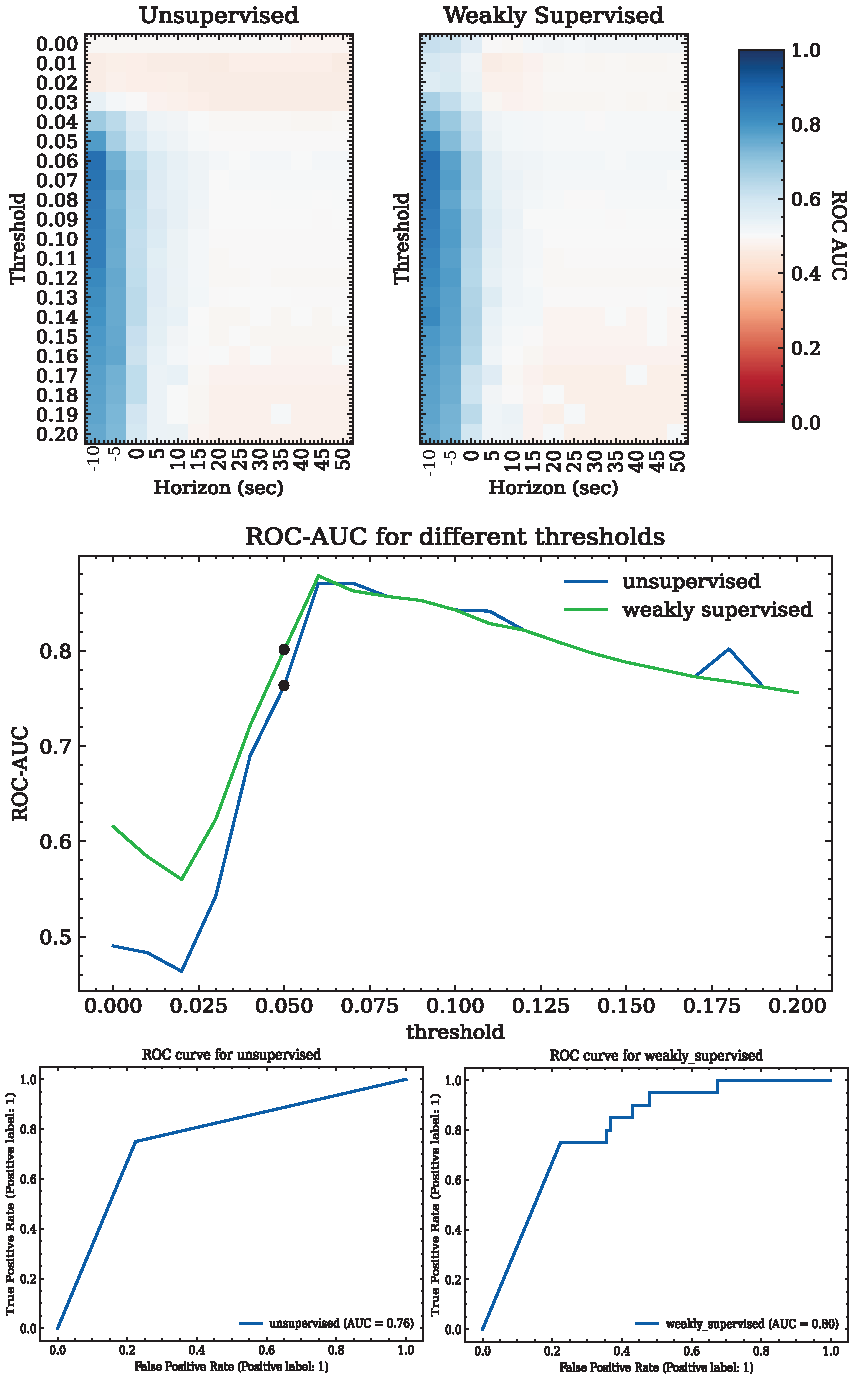
\includegraphics[width=\floatwidth]{c3Bsle/Figs/bsle/roc_grid.pdf}
    \Caption{Empirical results}{AUC-ROC scores smoothly distributed in the hyper-parameter space of both the unsupervised and weakly-supervised models, showing a low risk of overfitting (top row). The ROC-AUC of the weakly supervised model is usually higher than the unsupervised model (middle). An ROC curve is shown for each model when the likelihood threshold parameter is set to $\alpha=0.05$ (bottom).}
    \label{fig:c3bsle:roc_grid}
\end{figure}


% \subsection{Methods for evaluating forecast skill}
% \NS[inline]{write about probabilistic forecast skill evaluation methods}


% \section{Configuring seizure alerts}

% Based on the posterior class probability $\prob(S \mid E, t)$, we will configure warning alerts.
% \NS[inline]{determine method to configure alerts (business decision)}


% \subsection{Bayesian model checking}
% \NS[inline]{write about Bayesian model checking}

% \subsubsection{Prior}

% \subsubsection{Seizure Likelihood Estimation}

% \subsubsection{Model validation}
% \subsubsection{Linear probing}
% % https://arxiv.org/pdf/1610.01644.pdf
% % https://arxiv.org/pdf/2002.05709.pdf
% % https://www.youtube.com/watch?v=HJn-OTNLnoE

% By fitting the SVM to a training set and scoring the predictive accuracy on a hold-out test set, we can quantify the linear separability of the dataset. This is used as a proxy for representation quality.


% In order to further demonstrate the distinguishability between the interictal and ictal states, we show in figure \ref{fig:5results:svm} that a linear-kernel SVM fit to the training set achieves 0.91 AUC on the test set in the single-channel case. The double-channel case scores higher.

% \begin{figure}[htb]
    \centering
    \begin{subfigure}[b]{0.5\floatwidth}
        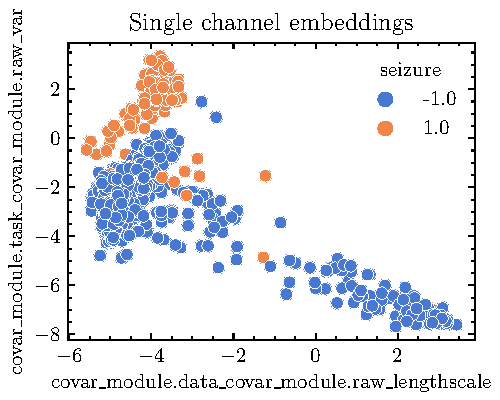
\includegraphics[width=\textwidth]{5Results/figs/svm/svm.pdf}
        \caption{decision boundary}
    \end{subfigure}
    \hfill    
    \begin{subfigure}[b]{0.5\floatwidth}
        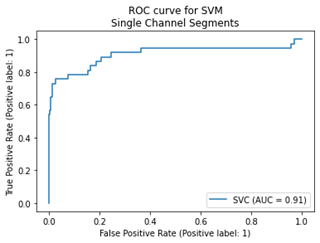
\includegraphics[width=\textwidth]{5Results/figs/svm/svm_roc.png}
        \caption{ROC curve}
    \end{subfigure}
    \hfill
    \Caption{Separability in the parameter space}{
	A support vector machine achieves 0.91 AUC-ROC on a held-out test set for single-channel segments.
	\protect \NS[inline]{remake seperability test figures}
    }
    \label{fig:5results:svm}
\end{figure}



% \subsection{AUC ROC, AUC PR}
% \begin{figure}[htbp]
  \centering
  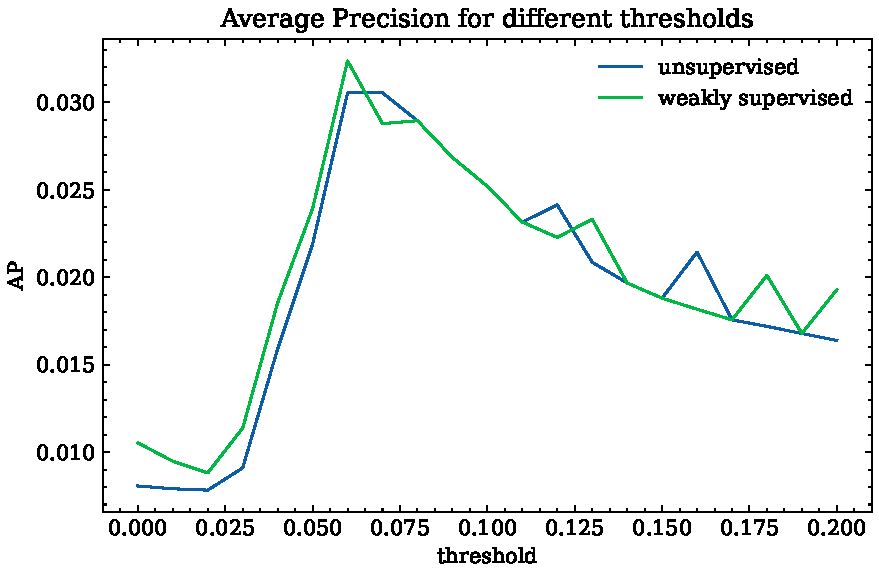
\includegraphics{5Results/figs/bsle/average_precision_score_for_thresholds.pdf}
  \caption{Average Precision scores (higher is better)}
\end{figure}
\begin{figure}[htbp]
  \centering
  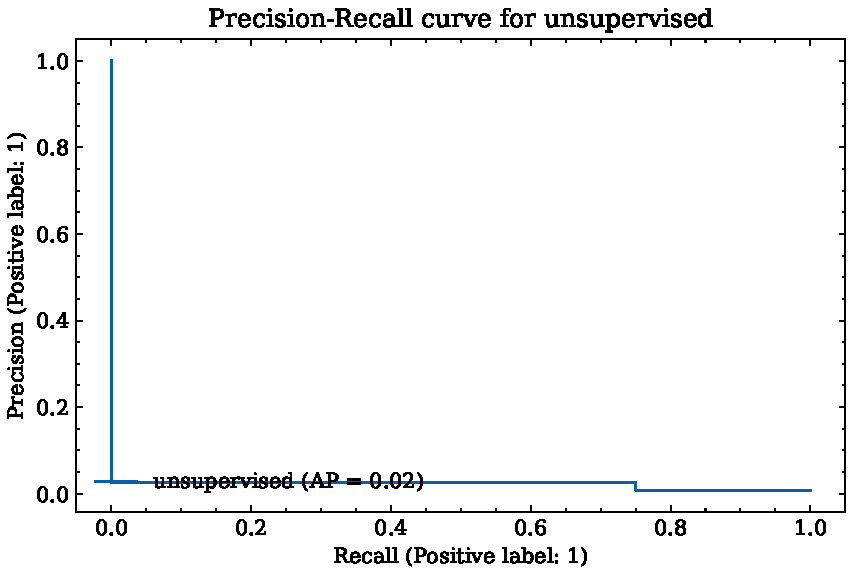
\includegraphics{5Results/figs/bsle/pr_auc_unsupervised.pdf}
  \caption{AP for unsupervised}
\end{figure}
\begin{figure}[htbp]
  \centering
  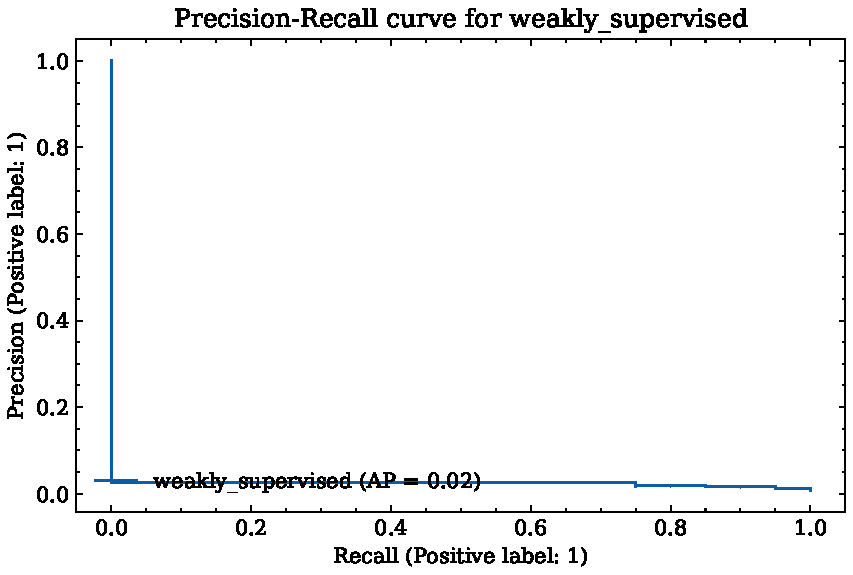
\includegraphics{5Results/figs/bsle/pr_auc_weakly_supervised.pdf}
  \caption{AP for weakly supervised (higher is better)}
\end{figure}
\begin{figure}[htbp]
  \centering
  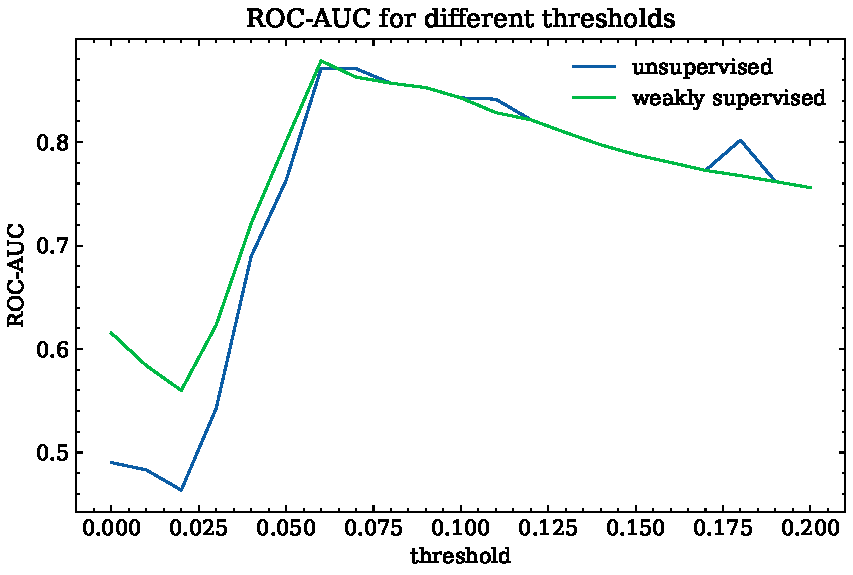
\includegraphics{5Results/figs/bsle/roc_auc_score_for_thresholds.pdf}
  \caption{ROC-AUC scores (higher is better)}
\end{figure}
\begin{figure}[htbp]
  \centering
  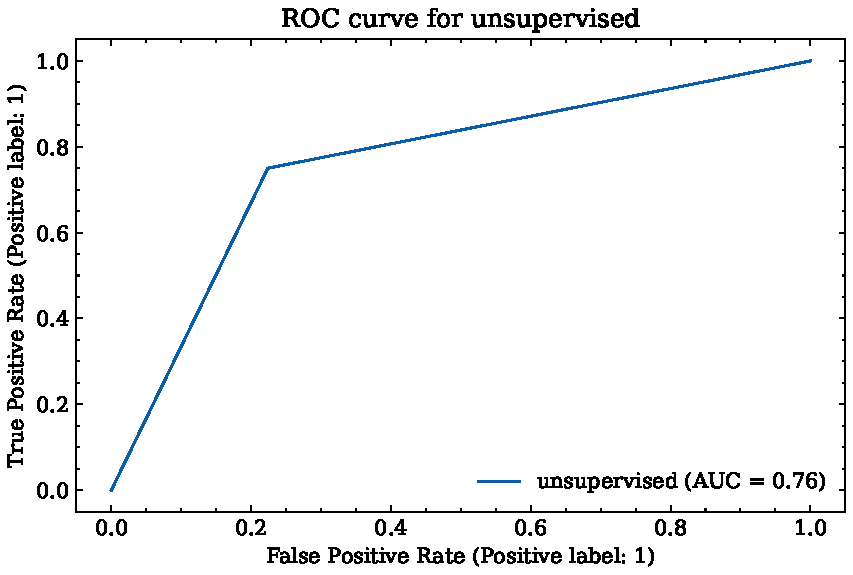
\includegraphics{5Results/figs/bsle/roc_auc_unsupervised.pdf}
  \caption{ROC for unsupervised}
\end{figure}
\begin{figure}[htbp]
  \centering
  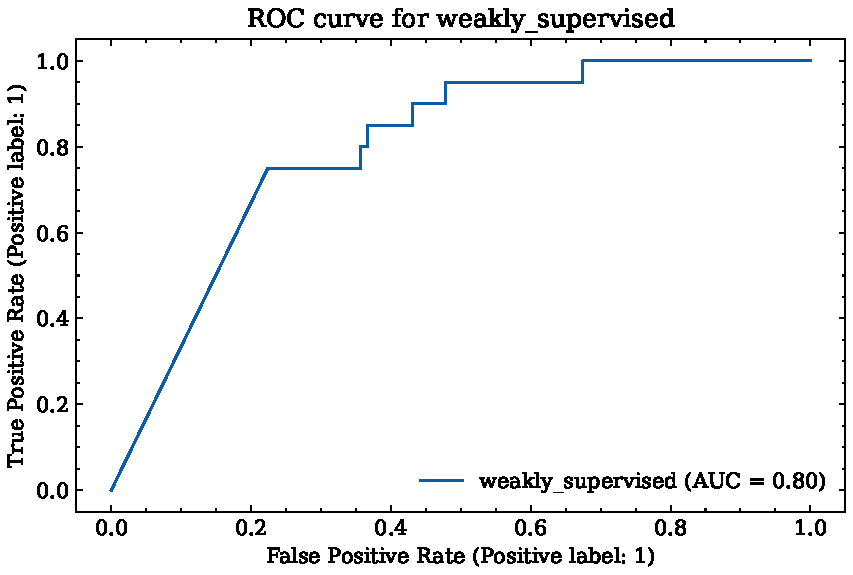
\includegraphics{5Results/figs/bsle/roc_auc_weakly_supervised.pdf}
  \caption{ROC for weakly supervised
  \NS[inline]{check which threshold made the roc curve fig and write it}
  }
\end{figure}
\begin{figure}[htbp]
\centering
  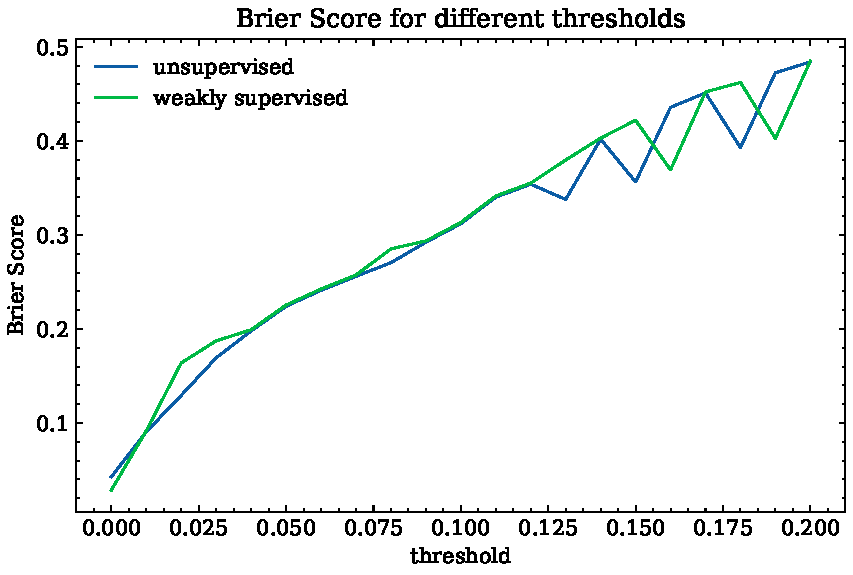
\includegraphics{5Results/figs/bsle/brier_score_for_thresholds.pdf}
  \caption{Brier scores (lower is better)}
\end{figure}
% \begin{figure}[htbp]
% \centering
%   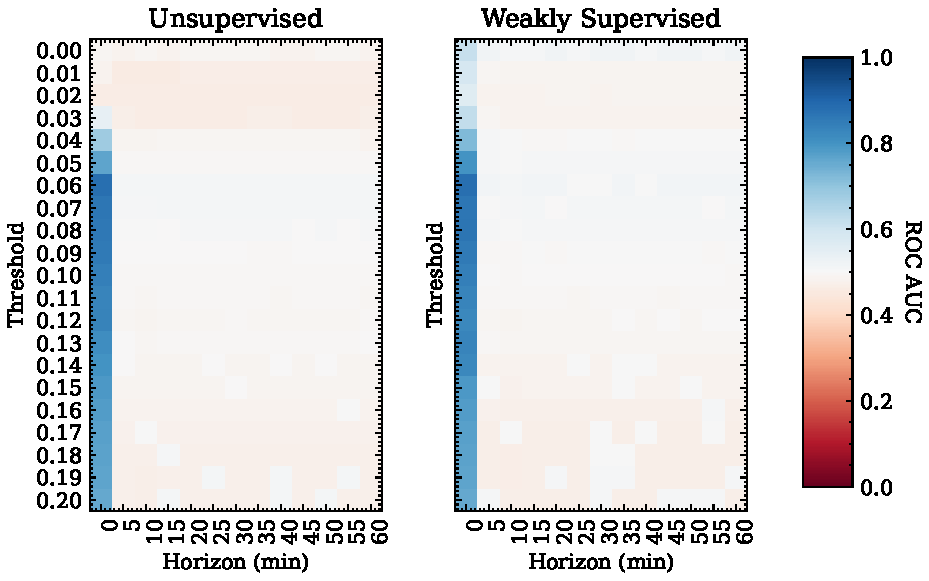
\includegraphics{5Results/figs/bsle/auc_roc_scores_for_thresholds_and_horizons_min.pdf}
%   \caption{AUC-ROC Heatmap for minutes time scale}
% \end{figure}
\begin{figure}[htbp]
\centering
  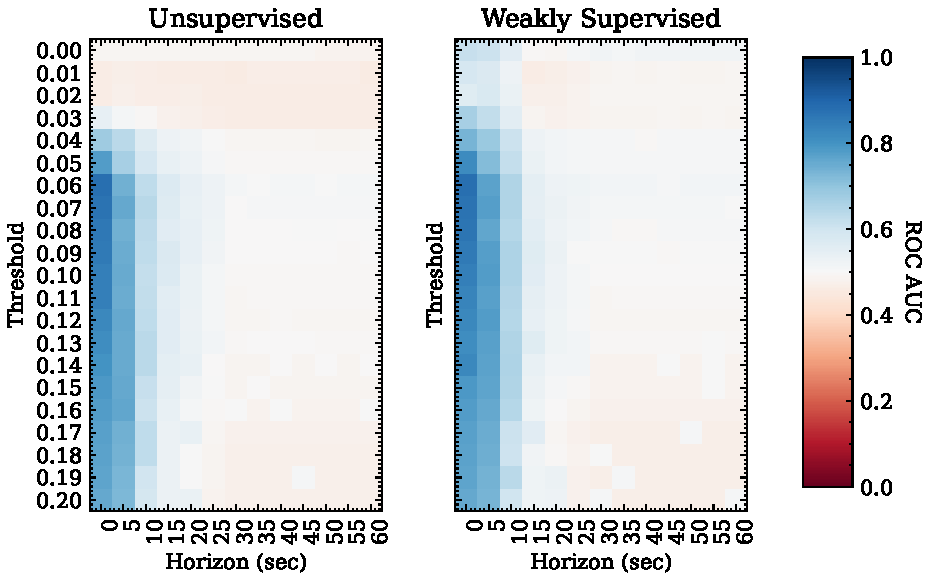
\includegraphics{5Results/figs/bsle/auc_roc_scores_for_thresholds_and_horizons_sec.pdf}
  \caption{AUC-ROC Heatmap for seconds time scale}
\end{figure}
% \Caption{Embedding of EEG}{}
% \label{fig:5results:bsle}


 \newpage
\fi


%%%%%%%%%%%%%%%%%%%%%%%%%%%%%%%%%%%%%% Chapter 4 - Conclusion %%%%%%%%%%%%%%%%%%%%%%%%%%%%%%%%%%%%%% 

\ifFULL
    \cleardoubleoddpage
    % =========================
\chapter{Conclusion}
\label{ch:4conclusion}
% =========================
The methods shown to work in this thesis are just instances of general approaches to seizure prediction. The pattern recognition approach, presented in chapter \ref{ch:2deterministic}, was selected because of its predominance in the reported literature and its prevalence in top-scoring competition submissions \cite{kaggle2014contests}. The probabilistic inference approach, presented in chapter \ref{ch:3Bsle}, was selected as a less-traveled alternative, which is compared and contrasted to the former approach.

The pattern recognition approach consists of labeling the entire dataset, and then training classifiers to discriminate between preictal and interictal segments. We explore this approach with off-the-shelf classifiers on the Epilepsiae \cite{ihle2012epilepsiae} dataset. To the best of our knowledge, chapter \ref{ch:2deterministic} is the first report to show that simple classifiers and nonlinear feature sets, such as those found in \cite{mirowski2009classification}, work also for noninvasive scalp EEG. The Linear SVM achieved above chance performance on all feature sets, with AUC-ROC scores in the range 0.65-0.96. Although the pattern recognition approach has delivered promising results and found widespread public interest in competitions, it faces limitations which inhibit it's development into practical appliances. One such limitation is the reliance on expert labels, which does not scale feasibly with the amount of EEG data.


The research question addressed in the second part of the thesis is, how can we formulate the task of seizure forecasting as a Bayesian inference problem? We answer this by proposing such a formulation, namely the Bayesian Seizure Likelihood Estimator, and evaluate it for both prediction and detection. This formulation utilizes the assumptions that seizures are rare, to identify rare events with a high likelihood for a seizure event, without the need for expert labels. 

The Bayesian framework is general in the sense that each of the likelihood, prior and evidence functions can be estimated independently, and then combined through multiplication. In the BSLE implementation, the likelihood function is constructed as a density-estimation-based novelty detector. We experiment with two options for the prior function: either constant mean seizure-rate values, for a fully unsupervised model, or a cyclical base-rate prior for a weakly supervised model.

We evaluate both types of models on a long-term iEEG recording from a canine with epilepsy. We discover that our method achieves ROC-AUC scores of 0.88 for both the unsupervised and weakly supervised modes after hyper-parameter tuning, and that for all $\alpha$-threshold values lower than 0.06, the weakly supervised model has higher ROC-AUC scores than the unsupervised model. Although this framework is suitable in theory for prediction as well as detection by choice of the horizon parameter, the empirical results (figure \ref{fig:c3bsle:roc_grid}) show that the method's ROC-AUC scores fall down to chance levels for horizons larger than 0.5 seconds.


While the uniform prior gives equal seizure probabilities to any block of time, the cyclical prior provides time-varying seizure probabilities. \citet{karoly2017circadian} showed that the circadian seizure histogram improved seizure forecasting in humans. To the best of our knowledge, chapter \ref{ch:3Bsle} is the first report to show that the same prior improves seizure forecasting in canines with epilepsy. This is another ever-so-slight indication that seizures tend to follow cycles, an observation which has been reported many times \cite{karoly2021cycles}.

Although the method we proposed works well for seizure detection, there are some drawbacks. First, the spatial information of the EEG channels is disregarded, and the selection of two channels to embed was made arbitrarily. Further work should utilize better channel selection and modeling the spatio-temporal qualities of the channels for potentially improved results. Second, the preictal data was not distinguishable in the GP-hyperparameter space from the interictal data. This precluded the possibility of using the method for seizure prediction. However, it is likely that different feature extraction methods, such as the ones used in chapter \ref{ch:2deterministic}, will preserve this information and could replace the GP embedding procedure.

We hope that further attempts at seizure likelihood estimation will add to our work within the framework of probabilistic modeling. Future research directions should utilize recent advances in probabilistic programming languages and dynamic Bayesian inference. These methods could allow more complex inference procedures such as inferring subject-specific latent hyperparameters with full uncertainty quantification. In addition, the BSLE model could be extended to multiple levels of hierarchy, for example by modeling multiple subjects together or the same subject at different stages of treatment.

% \section{Evaluation plan}
% Proper examination of seizure timing algorithms must account for all types of classification errors and be considerate of the imbalanced nature of the data. It is also essential to be able to benchmark the new algorithm against existing methods. Perhaps above all, it is worthy to evaluate the algorithm's applicability to real-world scenarios. Therefore, we will report a set of standard evaluation metrics for both the deterministic and the probabilistic settings, and attempt to replicate the setting proposed in \cite{karoly2017circadian} as much as possible.

%%%%%%%%%%%%%%%%%%%%%%%%%%
% \chapter{Discussion}
% \label{ch:5discussion}
%%%%%%%%%%%%%%%%%%%%%%%%%%
% \thispagestyle{empty}
% \vspace*{\fill}

%%%%%%%%%%%%%%%%%%%%%%%%%%%%%%%%%%%%%
%%%%%%%%%%%%%%%%%%%%%%%%%%%

% Consider the problem of modeling statistically the interdependencies between real-time EEG signals ($E$) from the epileptic brain, co-occurring seizures events ($S$), and board-approved annotations ($A$), throughout time ($T$).

% Seizures are states of abnormal brain function, which are associated with unwanted symptoms such as involuntary muscle movements (e.g., limb jerking, convulsing), partial or complete loss of consciousness and memory relapses.
% Epilepsy is a condition in which unprovoked seizures occur recurrently. People suffering from epilepsy may also suffer from side effects such as stress, fear, and sleep disorder. Prolonged seizures are especially dangerous and can lead to sudden death. Moreover, the uncertainty regarding seizure occurrence is regarded as one of the most disturbing factors of the disease. 

% and an external stream of timestamps denoting seizure events, commonly provided by

% It is said that every statistician would turn to Bayes' Theorem when an informative prior is available, but that only a "Bayesian statistician" will attempt to use it to solve any problem, whatsoever \cite{gelman2008objections}. In this work we chose to utilize mainly Bayesian techniques

% \section{Future work}

% Our work introduces a multilevel probabilistic model for dataset annotations (see figure \ref{fig:c3bsle:bsle_net}). The model is inspired by the hypothesis that clinical annotations are very precise but not highly sensitive. That is, we propose to relax the reliance on annotations even further by modeling the notion that a proportion of actual seizures don't become recorded annotation.
% % explained by the annotator's reliance on video-footage or a lack of clinical symptom manifestations

% % Full Bayesian Seizure Annotation Model
\begin{figure}[H]

  \tikz{

    % nodes
     \node[obs] (e) {$e_{t}$};%
     \node[latent, above=of e, xshift=1cm] (s) {$s_{t}$}; %
     \factor[above=of s, yshift=0.75cm] {cox} {right:Cox$(\lambda_{\phi_i})$} {} {}; 
     
    \node[latent, left=of cox] (phi) {$\phi_i$};
    \node[obs, below=of s, xshift=1cm] (a) {$a_{t}$};%
    \node[latent, below=of a] (o) {$o_{t}$}; %
    \factor[left=of o, xshift=-1cm] {ber} {above:Ber$(p)$} {} {};
    
    % gates
    \gate[] {seen} {(a)} {o};
    
    % edges
     \edge {s} {e, a}
     \edge {ber} {o}
    %  \edge {o} {a}
     \edge {cox} {s}
     \edge {phi} {cox}
    
    % plates
    
    \plate[inner sep=10pt] {plate1} {(e)(a)(s)(ber)(o)} {time $t$}; %
    \plate[inner sep=10pt] {plate2} {(plate1)(cox)(phi)} {subject $i$}; %

    % text
     \node[text width=6cm, anchor=west, right] at (4,1)
     {
       \begin{alignat*}{3}
        \phi_i & \sim \mathcal{D}_{\phi_i} \quad && \text{// subject-specific params}\\
        \lambda & _{\phi_i} (t) \gets \text{prior}_{\phi_i} : \Rplus \to \Rplus \quad &&\text{// intensity function}\\
        s_t & \sim \text{Cox}(\lambda_{\phi_i}) && \text{// stochastic counting process}\\
        e_t & \mid s_t \sim \mathcal{D}_{E \mid S} && \text{// EEG conditioned on seizure var}\\
        o_t & \sim \text{Bernoulli}(p) && \text{// was the seizure observed?}\\
        a_t & \sim s_t \text{ if } o_t \text{ else } 0 && \text{// sample annotation}\\
       \end{alignat*}
     };
   }
 \Caption{Probabilistically Modeling Seizure Occurrence, EEG signal and Annotations across Time and Subjects}{The nodes represent random variables. The shaded nodes $e$ and $a$ represent the observed variables EEG and Annotations, respectively. The rest are latent variables, which can be inferred with Bayes' theorem. The plates represent levels of hierarchy along which the model is replicated, such as time or subject, and the arrows indicate causal direction.}
  \label{fig:c3bsle:bsle_net}
\end{figure}

% The model describes, in mathematical terms, the process by which seizure annotations are generated. The $\phi$ parameters control the shape of the individual's prior latent distribution. $\lambda(t)$ is the time-varying seizure base-rate, technically referred to as the intensity function of the Cox process. To account for unannotated seizures, each seizure event $s_t$ is dropped with a probability of $p$. This reflects annotators' missing sections of the EEG recordings, as well as sub-clinical seizures.

% \begin{figure*}[h]
% \begin{algorithm}[H]
% \caption{Seizure Annotation Model}
% \label{alg:ann_model}
% \begin{algorithmic}
% \State $k \sim \text{Exp}(1)$
% \State $\alpha[0,...,23] \gets 1$
% \State $W[0,...,23] \sim \text{Dir}(\alpha)$
% \State $\lambda(t) \gets \sum_{i=0}^{23} W[i] \cdot f_{v.M.}(t; i, k)$
% \State $s_t \sim \text{Cox}(\lambda)$
% \State $a_t = \text{ZeroInflated}(s_t, p)$
% \end{algorithmic}
% \end{algorithm}
% % https://tex.stackexchange.com/a/460920
% \caption{A generative model for seizure events and annotations}{More formally, the probability of obtaining an annotation $a_t$ at time $t$ is a zero-inflated seizure occurrence model. Sequentially, in bottom-to-top order, the seizure-occurrence model is a Cox process with a stochastic intensity function $\lambda(t)$. In turn, the intensity function $\lambda(t)$ is a mixture model of 24 von-Mises distributions, one for each hour of the day, in line with \cite{karoly2017circadian}. Finally, the weights $W$ and common spread $k$ parameters assume noninformative (i.e. Dirichlet and Exponential) priors.}
% \end{figure*}




% \NS[inline]{write about Cox process (a.k.a. Inhomogeneous Poisson processes)}


% \NS[inline]{make figure of inferring latent intensity from samples (empirical data}

% \NS[inline]{add posterior predictive W, k plots, simulated seizures.}
 \newpage
\fi

%%%%%%%%%%%%%%%%%%%%%%%%%%%%%%%%%%%%%% Chapter 5 - Discussion  %%%%%%%%%%%%%%%%%%%%%%%%%%%%%%%%%%%%%% 

\ifFULL
    \cleardoubleoddpage
    %%%%%%%%%%%%%%%%%%%%%%%%%%
\chapter{Discussion}
\label{ch:6discussion}
%%%%%%%%%%%%%%%%%%%%%%%%%%
% \thispagestyle{empty}
% \vspace*{\fill}
\epigraph{"The theory of probabilities is at bottom nothing but common sense reduced to calculus"}{---Pierre-Simon Laplace, \textit{Essai Philosophique sur les Probabilités}}

\NS[inline]{rewrite discussion. Points to include: (1) future work on hierarchical patient modeling}

The problem of automatic seizure detection is challenging, inducing many attempts over the years. In this work we attempted a probabilistic approach, relying on Bayes' rule to estimate the likelihood of a seizure given an EEG segment. We assumed that seizures are rare, which led us to a novelty-score-based likelihood. Following recent findings, we also assumed that seizures are approximately cyclical, taking this into account in our prior.

\showthe\textwidth

% It is said that every statistician would turn to Bayes' Theorem when an informative prior is available, but that only a "Bayesian statistician" will attempt to use it to solve any problem, whatsoever \cite{gelman2008objections}. In this work we chose to utilize mainly Bayesian techniques


Although the method we proposed works well, there are some drawbacks. First, the channel spatio-temporal location is disregarded, and the pairing (in the double-channel case) was made arbitrarily. Further work should utilize better channel selection and modeling the topographic qualities of the channels for potentially improved results.

Second, the model of normal EEG was fit using the segments from the Canine-epilepsy-dataset which were chosen for the Kaggle challenge. The class distribution differs from the true class distribution. To combat this discrepancy, we dropped the ictal segments and used only the interictal segments for the model of normality. Because ictal EEG is extremely less common than interictal EEG, we assume that using the interictal segments is a sufficiently close approximation of the natural distribution. Further studies should recalibrate the method based on the raw recordings in order to provide an even better estimate.

Thirdly, from the clinical perspective, the evaluation method is limited since the data originates from canines with naturally occurring epilepsy, instead of humans. Dogs with naturally occurring epilepsy show similar semiology to epilepsy in humans, but more work is required to validate this method on human EEG. 

In summary, we present an anomaly detection method based on Gaussian processes embeddings, and evaluate it on a seizure detection task. The method is significant because it is unsupervised, thus eliminated the need for costly annotators.
 \newpage
\fi

% remove section names from page headers
\ifPRINT
    \ihead{}
\else
    \rehead{}
    \rohead{}
\fi

%% Bibliography:
%%

\ifBIB
    \cleardoubleoddpage
    % \ifDRAFT
        % \bibliographystyle{apalike} %(author, year) when inline
%         \bibliographystyle{References/apalike-refs.bst} %(auther, year) with DOI, hyperlinks and many more goodies
    % \else
        \bibliographystyle{unsrtnat} %numbers only when inline
        % \bibliographystyleall{unsrtnat} %numbers only when inline
    % \fi
    
    \bibliography{References/ref}
    % \bibliographyall{References/ref}
    % \nocite{*}
    % \nobibliography{References/myref}
\fi


\begin{appendices}
        %\bookmarksetupnext{level=0}
        %\addappheadtotoc
        
%         \renewcommand{\thesection}{A.\arabic{section}}

%%%%%%%%%%%%%%%%%%%%%%%%%%%%%%%%%%%%%% Chapter 6 - Appendix A  %%%%%%%%%%%%%%%%%%%%%%%%%%%%%%%%%%%%%% 

\cleardoubleoddpage
% =========================
\appendix


%%%%%%%%%%%%%%%%%%%%%%%%
\chapter{Density estimation: mathematical derivations}
\label{apx:DEMath}
\section{Embedding time series with Gaussian processes hyperparameters}
\label{apx:GPEmbed}
A Gaussian process (GP) \cite{rasmussen2006cki} is \emph{a collection of random variables, any finite number of which have a joint Gaussian distribution}.

A Gaussian process $f(x)$ is fully specified by a mean function $\mu(x)$ and a covariance function, or a kernel, $k(x,x')$, by-way-of:

\begin{align}
    m(x) &= \E[f(x)] \\
k(x,x') &= \E[(f(x)-m(x))(f(x')-m(x')]
\end{align}

And it is denoted:

\begin{align}
    f(x) \sim \mathcal{GP}(m(x), k(x,x'))
\end{align}

In this work we will take the mean function to be zero.

\subsubsection{parameter estimation (inference)}
Gaussian processes are commonly used for time series modeling with machine learning. To see why this makes sense, imagine the input $x$ is the time point, and the output $f(x)$ is the time series value at time $x$. Computationally, this is made feasible by evaluating the function's values at a finite number of points of interest.
Using optimization techniques, the model's hyperparameters are inferred to match observed data by maximizing the likelihood function $p(f(x) \mid \Vec{\theta})$ (termed maximum likelihood estimation, or MLE). The learned hyperparameters capture global evolutionary dynamics of the time series.

%  (see figure \ref{fig:3methods:posterior_draws} in the Methods section)

\subsubsection{The Matérn class of covariance functions}
The Matérn class of covariance functions is given by:

\begin{align}
    k_{Matern}(x,x') = \frac{2^{(1-\nu)}}{\Gamma(\nu)}(\sqrt{2\nu}d)^\nu K_\nu (\sqrt{2\nu}d)
\end{align}

Where:
\begin{itemize}
    \item $d = (x-x')^T \Phi^{-2} (x - x')$ is the distance between $x$ and $x'$ scaled by the \emph{lengthscale} parameter $\Phi$.
    \item $\nu$ is a smoothness parameter. In this work, it is taken to be $\frac{3}{2}$.
    \item $K_\nu$ is a modified Bessel function.
\end{itemize}

\subsubsection{Multitask Gaussian processes}
In case $f(x)$ is a vector function, multiple output functions are modeled in conjunction for the same input values, so-called multitask Gaussian process modeling. In this case, given inputs $x$ and $x'$, and tasks $i$ and $j$, the covariance between two datapoints and two tasks is given by:

\begin{align}
\label{eq:2background:multitask}
    k([x,i], [x',j]) = k_{inputs}(x,x') \cdot k_{tasks}(i,j)
\end{align}

Where $k_{inputs}$ is a standard kernel (e.g., Matérn) that operates on the inputs, and $k_{tasks}$ is a lookup table containing inter-task covariance. This is akin to capturing the inter-channel synchronicity with manually engineered features (see section \ref{sec:c2:features}).


\subsubsection{Gaussian process parameters embedding}
Inference of Gaussian process (GP) parameters is a well-documented approach to modeling time-series data \cite{rasmussen2003gaussian}. The extension to multitask GPs enables modeling of multivariate time-series, such as the case of multi-lead EEG signals.

% \begin{figure}[htbp]
    \centering
    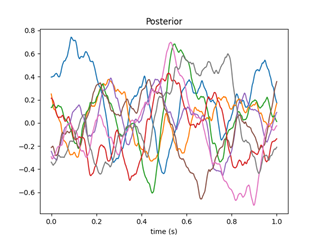
\includegraphics[width=0.4\floatwidth]{3Methods/Figs/GP/posterior_draws.png}
    \Caption{Embedding EEG with GP hyperparameters}{
	Posterior draws from a Gaussian process fit to maximize the likelihood of an observed single-channel EEG segment.
	\protect \NS[inline]{replace with vectorized image}
	\protect \NS[inline]{add original sample}
    }
    \label{fig:3methods:posterior_draws}
\end{figure}


For each EEG segment $x$, the preprocessing steps include:

\begin{enumerate}[label=\roman*]
    \item Normalizing $x$ by subtracting the mean and dividing by the standard deviation of the training set.
    \item initializing a GP model with zero mean, a scaled Matérn-1.5 kernel, and a rank-1 multitask covariance kernel.
    \item Optimizing the model's parameters to obtain a maximal marginal log-likelihood (details in appx. \ref{apx:GPTraining}).
\end{enumerate}

The optimized model's parameters $\theta$ are persisted and used henceforth to represent the original EEG segment $x$.


\section{Gaussian Mixture Models}
\label{apx:GMM}
Gaussian mixture models \cite{theodoridis2015machine} are used to model the distribution of an unknown set of vectors $\{x\} \subseteq \mathbb{R}^l$ as a linear combination (i.e., a mixture) of different Gaussian distributions, that is,

\begin{align}
    p(x) = \sum_{k=1}^{K}p_kp(x \mid k; \zeta_k)
\end{align}

where $\{\zeta_k\}$ parametrize the individual Gaussian distributions:
\begin{align}
    p(x \mid k ; \zeta_k) = p(x \mid k; \mu_k, \sigma_k) = \mathcal{N}(x \mid \mu_k, \sigma_k)
\end{align}

Fitting the model (e.g. via expectation maximization) provides an approximation $\hat p(x \mid k; \zeta_k)$ of the dataset's underlying pdf, which is an estimate of the data-distribution of the GP-hyperparameters $P(E \mid D)$


%%%%%%%%%%%%%%%%%
\chapter{GP embedding: training details}
\label{apx:GPTraining}

% =========================
For dimensionality reduction of an observed EEG segment, we performed exact inference of the GP parameters maximizing the observation likelihood, using the GPyTorch and PyTorch Lightning frameworks \shortcites{gardner2018gpytorch} \cite{gardner2018gpytorch, Falcon_PyTorch_Lightning_2019}.

More formally, in fitting the Gaussian processes to the EEG samples we carried out exact Type-II Maximum Likelihood Estimation for each sample. This means optimizing the model's hyperparameters (mean module, covariance module, etc.) w.r.t maximization of the \emph{marginal log likelihood} (MLL) of the given data $\mathbf{E, t}$:

\begin{align}
    \theta \gets \argmax_\theta p_f(\mathbf{E} \mid \mathbf{t}) = \int p(\mathbf{E} \mid f(\mathbf{t})) p(f(\mathbf{t}) \mid \mathbf{t}) df
\end{align}

where $f \sim \mathcal{GP}(\mu, K)$ is the modeled signal before adding the homescedastic Gaussian noise, and $\theta$ is the set of parameters to be optimized. See code for implementation details.

\begin{table}[h]
\begin{tabular}{ |p{3cm}||p{5cm}||p{5cm}| }
 \hline
 \multicolumn{3}{|c|}{GP \& inference (training) configuration details} \\
 \hline
  &Parameter& Value \\
 \hline
\multirow{5}{3cm}{GP params} & mean module & zero mean\\
&covariance module& scaled Matérn-1.5 kernel\\
&task covariance rank& 1 \\
&number of tasks& 2   \\
&likelihood (noise model)&Gaussian (homoscedastic)\\
\hline
\multirow{4}{3cm}{Training params}& optimizer &Adam\\
&learning rate& 0.01 \\
&max. number of epochs & 1000\\
&patience (early stopping)&8 \\
 \hline
\end{tabular}
\caption{The GP parameters and training parameters used in our experiments.}
\label{table:GPTraining}
\end{table}


        
\end{appendices}
% %Appendix with no toc page number and no prefix
% %https://tex.stackexchange.com/a/411021/199031
% \ifFULL
%     \ifAPPENDIX
%         \cleardoubleoddpage
        
%     \fi
% \fi

% \ifLINENO
%     \nolinenumbers
% \fi

\pagestyle{plain} %no header, with pagenum

%%%%%%%%%%%%%%%%%%%%%%%%%%%%%%%%%%%%%%%%%%%%%%%%%%%%%%%%%%%%%%%%%%%%%%%%%%%%%%%%
%% Index:
%%
% \ifFULL
%     \cleardoubleoddpage
%     \printindex
%     % \thispagestyle{empty} %no pagemark footer here
%     \blankPageWithoutFooter
% \fi

%%%%%%%%%%%%%%%%%%%%%%%%%%%%%%%%%%%%%%%%%%%%%%%%%%%%%%%%%%%%%%%%%%%%%%%%%%%%%%%%
%% Hebrew cover:
%%
\ifFULL
    \ifHEBCOVER
        \cleardoubleevenemptypage
        % \blankPageWithoutFooter
%         
\includepdf[pages=last-1,addtotoc={1,chapternonum,0,Hebrew cover,hebcover}]{Hebrew/hebCover.pdf}

%---------------------------- Reminder including a PDF document to TOC (see macros)
% includepdf syntax:
%     addtotoc={⟨page number⟩,⟨section⟩, ⟨level⟩,⟨heading⟩,⟨label⟩}
%     addtolist={⟨page number⟩,⟨type⟩,⟨heading⟩,⟨label⟩}
%   \IncludeMyPDF
%   {1} %  page number to be included
%   {0.9} % scale
%   {true} %   landscape = true or false
%   {false} %  turn = true or false
%   {subsection,2} % level in TOC: section, subsection, subsubsection + level 1,2,3
%   {TitleTOC} %  heading for TOC / list 
%   {Label} %   label: label-toc-#7, label-list-#7, #7-target for hyperlinks
%   {table} %   addtolist = table or figure
%   {mindmaps.pdf} %  file
        % Add the hebrew pages in reverse order, and add the hebrew abstract to ToC
        \def\hebabstractpage{3}
        
        \IncludeMyPDFinReverse
        {\hebabstractpage}
        {1}
        {false}
        {false}
        {chapternonum, 1}
        {Hebrew Abstract}
        {fig:hebCover}
        {figure}
        {Hebrew/hebCover.pdf}

        % 
\includepdf[pages=last-1, noautoscale, addtotoc={\hebabstractpage, chapternonum, 0, Hebrew Abstract, hebabstract}]{Hebrew/hebCover.pdf}
        
        % Add a PDF bookmark to the hebrew cover
        \bookmark[startatroot, named=LastPage, level=0]{Hebrew Cover}
    \fi
\fi

\ifLISTFIGS
    \listoffigures
\fi

\end{document}
